\documentclass[12pt, twoside]{report}
\usepackage[a4paper,width=150mm,top=25mm,bottom=25mm,bindingoffset=6mm]{geometry}
\usepackage[utf8]{inputenc}
\usepackage{fancyhdr}
\pagestyle{fancy}
\usepackage{graphicx}
\graphicspath{ {images/} }
\usepackage{amsmath}
\usepackage{mathrsfs}
\usepackage{listings}
\usepackage{caption}
\usepackage{subcaption}
\usepackage{commath}
\usepackage{hyperref}
\usepackage{url}
\usepackage{xcolor}
\usepackage{textcomp}
\usepackage{float}
\usepackage{listings}
\usepackage[backend=biber,sorting=none,style=numeric-comp]{biblatex}
\usepackage[linesnumbered,lined,boxed,commentsnumbered]{algorithm2e}

% Packages from derivations_fullproblem.tex
\usepackage[squaren]{SIunits}
\usepackage{a4wide}
\usepackage{array}
\usepackage{cancel}
\usepackage{amsfonts}
\usepackage{amssymb}
\usepackage{enumerate}
\usepackage{physics}

% Ref file
\addbibresource{ref.bib}

% References ----------------------------------------------------------------- %
\newcommand{\Fig}[1]{Fig.\ \ref{fig:#1}}
\newcommand{\fig}[1]{Fig.\ \ref{fig:#1}}
\newcommand{\eq} [1]{Eq.\ (\ref{eq:#1})}
\newcommand{\Eq} [1]{Eq.\ (\ref{eq:#1})}
\newcommand{\tab}[1]{Table \ref{tab:#1}}
\newcommand{\Tab}[1]{Table \ref{tab:#1}}

% Parameters for displaying code.
\lstset{language=C++}
\lstset{basicstyle=\ttfamily\small}
\lstset{frame=single}
\lstset{keywordstyle=\color{red}\bfseries}
\lstset{commentstyle=\itshape\color{blue}}
\lstset{showspaces=false}
\lstset{showstringspaces=false}
\lstset{showtabs=false}
\lstset{breaklines}

\title{{Weak and strong interacting Bose gases with Restricted Boltzmann Machine}\\
{\large University of Oslo}\\

\includegraphics[scale=1.0]{uio_logo2.eps}
}
\author{Kari Eriksen}
\date{Desember 2019}

\begin{document}

\maketitle

\chapter*{Abstract}
Abstract goes here

\tableofcontents
 
%\chapter*{Dedication}
 
%\chapter*{Declaration}

%\chapter*{Acknowledgements}

%\chapter{Introduction}
%\input{chapters/introduction}

\part{Theory}
 
\chapter{Many-body quantum theory}
Some introduction containing historical information and stuff, and motivation for this section. 
Configuration interaction, Many-body perturbation theory, Coupled-cluster 
Electron correlation,
Large systems, few with a corresponding analytical solution, in most cases we must turn to numerical tools. 
Solving the Schrödinger equation, analytical and now numerical

Many-body algebraic methods originate from quantum field theory \cite{shavitt2009many}

\section{Classical Mechanics}

In classical mechanics a particles state is described by two variables, the particles position and its momenta. For a system of N particles the position and the momentum, $q = (\vec{r}_1, \cdots,\vec{r})_N$ and $p = (\vec{p}_1, \cdots,\vec{p}_N)$, together form a point $\xi(q, p)$ in a two-dimensional \textit{phase space} $\in \mathbb{R}^{2 \cdot n}$ \cite{kvaal}. The phase space contains all the possible values for these two variables.
The state variables are governed by \textit{Hamilton's equation of motion},

\begin{align}
\dot{q} &= \frac{\partial}{\partial p} \mathscr{H} (q, p) \\
\dot{p} &= -\frac{\partial}{\partial q} \mathscr{H} (q, p),
\end{align}

where $\mathscr{H}$ is the $\textit{Hamiltonian}$, an operator that we interpret as the total energy of the system. To see this we write out a special case within the classical Hamiltonian dynamics

\begin{align}
\mathscr{H}(q,p) &= \mathscr{T}(p) + \mathscr{V}(q) + \mathscr{W}(q) \\
&= \frac{1}{2m} \sum^N_{i=1} |\vec{p}_i|^2 + \sum^N_{i=1} v(\vec{r}_i) + \frac{1}{2} \sum^N_{i \neq j} w(r_{ij})
\end{align}.

This is the Hamiltonian for N particles of mass m, with inter-particle reaction through the force of a central potential $w(r_{ij}) = |\vec{r}_i - \vec{r}_j|$, moving in an external potential field $v(\vec{r})$. We recognize the first term as the $\textit{kinetic energy}$, the second term as the $\textit{external potential energy}$, and the final term as the $\textit{interaction energy}$.

\section{Quantum Mechanics}

In ordinary quantum mechanics an observable is a linear operator acting on a Hilbert space. Position operator and momentum operator, other observable quantities like angular momentum, energy, and so on, are linear operators constructed out of linear combinations of products of the position and momentum.\cite{kvaal}
Atomic units, all equal 1.
Hamiltonian 

\subsection{Canonical quantization}

In order to move from the classical Hamiltonian description of a particle system to the quantum mechanical description we now look at canonical quantization. 
In classical mechanic we described the state of a system as a point in phase space. In quantum mechanics however the state is a vector containing all information about the system. The $\textit{quantum state}$, $\psi$, is a complex-valued vector state in an infinite $\textit{Hilbert space}$, i.e. a complete vector space with an inner product. The inner product will represent a complex number that link two elements within the vector space. 

Where the measurement of variables in the classical case was given through an observable $\omega(q, p)$, the quantum observable is an $\textit{Hermitian}$ (self-adjoint) operator $\Omega$. The operators value in the state $\psi$ is called an $\textit{expectation value}$.
In quantum mechanics we work with expectation values, this because we can not measure a particles quantities accurate. We do not know where the particles will be at a given time, so we work with probabilities. We can measure the probability of a particle being at a certain place at a certain time. So the expectation value tells us the likeliest position or momentum of a particles state. 
Given a system of identical particles, what we work with in quantum mechanics, they have position. But also an extra internal degree of freedom, spin. Coordinate $x = (\vec{r}, s)$. Then our state $\psi(x_1, \cdots , x_N)$ is the wave equation that depends on all coordinates and $(x_1, x_2, \cdots , x_N) \in X^N$ is a point in the configuration space of N particles. 

\begin{equation}
\expval{\Omega} = \expval{\hat{\Omega}}{\psi} = \int \psi (x_1, \cdots , x_N)^\ast [\hat{\Omega} \psi (x_1, \cdots, x_N)] dx_1 \cdots dx_N
\end{equation}

We can obtain all physical properties of the system through the state $\psi$.
So how do we move from the classical case to the quantum mechanical one? Canonical quantization is a procedure where we rewrite the classical coordinates $\xi(q, p)$ to operators $(\hat{q}, \hat{p})$. This is done through the canonical commutation relations.

\begin{equation} \label{eq:commutation}
\{q_i, p_j\} = \delta_{ij} \Longrightarrow [\hat{x}_i, \hat{p}_j] = i \hbar \delta_{ij}
\end{equation}

The left side of this equation tells us that our coordinate system in the classical case is canonical. We turn the Poisson brackets in to commutation relations to determine the new operators. 
The new 

\begin{equation}
\hat{x}\psi = x \psi \ \ \text{and} \ \ \hat{p} \psi = -i \hbar \frac{\partial \psi}{\partial x}
\end{equation}

But the Hilbert space is also a part of the solution and is often chosen as the space of square-integrable function, $L^2$. This is convenient since the state $\psi$, in quantum mechanics interpreted as the wave equation, has a associated probability given by itself squared,

\begin{equation}
P(x_1, \cdots, x_N) = |\psi(x_1, \cdots, x_N)|^2.
\end{equation}

Where $P(x_1, \cdots, x_N)$ is the probability of the system being in its given state. Since the particles has to be somewhere, the sum over all probabilities must equal one, 

\begin{equation}
\int_{X^N} |\psi(x_1, \cdots, x_N)|^2 d x_1 \cdots d x_N = 1.
\end{equation}

The wave function is a map, a Fourier transformation? 

\begin{equation}
\psi : X^N \longrightarrow \mathbb{C}
\end{equation}

\subsection{Canonical transformation}

A one-to-one algebra morphism of an observable, u, onto itself leaving the canonical commutation relations invariant. The canonical transformation is a map, $u \rightarrow u$ 

Suppose $X = (Q, P) = F(\xi) = F(q, p)$ is a differentiable coordinate change such that $F^{-1}$ exits and is differentiable, and such that $\{Q_j, P_k\} = \delta_{jk}$. This is called a canonical transformation

properties satisfying 

-linearity
-invariance
-product conserving (s. 175 MBBS)

\subsection{Second quantization}

Second quantization formalism is designed expressly for calculating matrix elements of operators between wave functions of the form 

\begin{equation}
\psi (r_1, r_2, \cdots, r_N) = c_N \sum_{sym} \phi_1(r_1) \phi_2(r_2) \cdots \phi_N(r_N)
\end{equation}

Now the particles themselves are discrete quanta created and destroyed with creation and annihilation operators

Position operator 

\begin{equation}
[\hat{r_i} \psi](x_1, \cdots, x_N) = r_i \psi (x_1, \cdots, x_N) 
\end{equation}

Momentum operator 

\begin{equation}
[\hat{p_i} \psi](x_1, \cdots, x_N) = -i \hbar \nabla_i \psi (x_1, \cdots, x_N) 
\end{equation}

Fock space

\subsection{symmetri}
Symmetric states, bosons. Why they differ from fermions.
How does this effect the wave equaiton

\section{The Schrödinger equation}

With a change of basis we can take the Heisenberg picture of quantum mechanics and move to the Schrödinger formalism where the states evolve in time and the operators are constant. 

\begin{equation}
i \hbar \frac{\partial}{\partial t} \ket{\psi(t)} = \hat{H} \ket{\psi(t)}
\end{equation}

We are searching for the ground state of our system, which means it is sufficient to look at the time-independent Schrödinger equation.

\begin{equation}
\hat{H} \psi(x_1, x_2, \cdots, x_N) = E \psi (x_1, x_2, \cdots, x_N)
\end{equation}

The many-body Hamiltonian (s. 12) 

one-body operator  

two-body operator

\section{The Harmonic Oscillator}


\chapter{Dilute Bose Gases}
The area/study of dilute Bose gases has been a field of research with great many discoveries over the last decades. The fact that microscopic quantum phenomena can be observed at a macroscopic level, compared to an atomic one, makes it an interesting subject in it self. With the improvement of laser cooling techniques there has been an explosion of discoveries and verification of theories of dilute Bose gases. Some of which include cold atomic gases of Rubidium-87, Sodium-23 and Lithium, (reference) 1995.

In dilute gases the scattering length is shorter than the inter-particle spacing. If we compare the molecule density in air at room temperature and atmospheric pressure which is $10^{19}$ cm$^{-3}$ to the density of a dilute gas at about $10^{14}$ cm$^{-3}$, the difference is enormous.

However, in order to observe quantum effects at such low densities, we must require low temperatures. Helium liquid must be cooled to the order of 1 K, absolute zero in order for effects to occur. This compared to electrons in metals which show quantum effects below the Fermi temperature, $10^4 - 10^5$ K. 
For the atomic nuclei the density is so high that degeneracy happens at temperature close up to $10^{11}$ K.

Bose-Einstein condensation in dilute gases occurs when the temperature is so low that $\lambda_T$, the thermal de Broglie wavelength, is comparable to the mean interparticle spacing, $n^{-1/3}$ \cite{BECCondInDilute}.

\begin{equation}
\lambda_T = \left( \frac{2 \pi \hbar^2}{m k T} \right)^{1/2}
\end{equation}

If $T$ is high then $\lambda_T$ is small, and the gas behaves classically. 

Working with dilute gases gives us the opportunity to approximate the system by a mean-field approach using Hartree-Fock theory. This is the basis of the Gross-Pitaevskii equation, the foundation of the studies of the Bose-Einstein condensate. It is an equivalence to the Schrödinger equation.

Maybe specify some constants if that is necessary. 

Application in condensed-matter physics, fluid mechanics, atomic and nuclear physics.

\section{Bose-Einstein Condensate}

The Bose-Einstein condensate (BEC) is the state of a dilute Bose gas at low temperatures at which most of the particles in the gas all resides the same quantum state. This was predicted by Albert Einstein in 1925 after taking the work of Satyendra Nath Bose, studying the statistics of photons, further. He considered a non-interacting gas of bosons at low temperature and concluded that the particles could all be found in the lowest-energy single-particle state. Together with Bose he formed the foundation of Bose-Einstein statistics which describes the statistical distribution of bosons. Before looking closer at the statistics in thermodynamics it can be practical to explain what a boson is.

\subsection{Bosons and fermions}
Bosons are particles with integer spin. They can be fundamental particles like the photon or gluon. But also composite particles like mesons or the stable isotope of the helium atom, $^4\text{He}$. They posses the ability to occupy the same quantum state, unlike fermions which are particle of half-integer spin. Fermions include all quarks and leptons, but as bosons they can also be composite particles, like $^3\text{He}$. They underlay the Pauli exclusion principle. It states that two or more identical fermions can not occupy the same quantum state. 
The typical example being two electrons occupying the same orbital in an atom must have opposite spin quantum number as they have same quantum numbers otherwise. 
This principle leads to fermions being governed by the Fermi-Dirac statistics and bosons by the Bose-Einstein statistics. 

% Add some single particle basis vectors
% explain the symmetric and antisymmetric solutions?

We will come back to this, but first, lets look at one of the most important formulas in statistical mechanics. 

\subsection{Particle statistics}

OBS: lese om partition function i boka hjemme!


Picture a system in thermal equilibrium with a reservoir with temperature T, a canonical system. Then we know from thermal physics that the probability of finding a system in any particular microstate $s$ with energy $E(s)$ is given by \eqref{eq:prob_boltzmann}.

\begin{equation} \label{eq:prob_boltzmann}
P(s) =  \frac{1}{Z} e^{-E(s)/kT}    
\end{equation}

The exponent is the Boltzmann factor, $e^{-E(s)/kT}$, where $k$ is the Boltzmann constant and $T$ the temperature of the reservoir. $Z$ is called the \textit{partition function}, the sum over all Boltzmann factors i.e. the sum over all states. This is easily seen if we use the fact that the sum of all possibilities must equal 1. The particle must be in one of the states. 

%Average values: page 230 thermal physics

\begin{equation}
1 = \sum_s P(s) = \sum_s \frac{1}{Z} e^{-E(s)/kT} = \frac{1}{Z} \sum_s e^{-E(s)/kT}
\end{equation}

If we now look at a system where the system is allowed to exchange particles with the environment as well as the energy, the factor in the exponential changes. And we end up with the Gibbs factor. 

\begin{equation}
\text{Gibbs factor} = e^{-[E(s) - \mu N(s)]/kT}
\end{equation}

We are now looking at a grand canonical system, and the partition function from before is now a grand partition function.
Now we can calculate the probability of a system containing N particles being in the state s(N) with corresponding energy E(s).
$\mu$ being the chemical potential of the reservoir that is effectively constant, T also constant.

\begin{equation}
P(n) = \frac{1}{Z} e^{-n(\epsilon - \mu)/kT}
\end{equation}

We want to find the average number of particles being in one energy state $\epsilon_{\mu}$, i.e. the distribution of particles over energy states. Lets consider the probability of a particle occupying a single-particle state. 

If we begin looking at fermions, we know they obey the Pauli exclusion principle, and the grand partition function for the one particles is given by \eqref{eq:partition_fermion}.

\begin{equation} \label{eq:partition_fermion}
Z = 1 + e^{-(\epsilon - \nu)/kT}
\end{equation}

Since the particle can either occupy the state or not we get the following.

\begin{equation}
\overline{n} = \sum_n n P(n) = \frac{e^{-(\epsilon - \mu)/kT}}{ 1 + e^{-(\epsilon - \mu)/kT}} = \frac{1}{e^{-(\epsilon - \mu)/kT} + 1}
\end{equation}

Forklar denne funksjonen...

\begin{equation}
\overline{n}_{FD} = \frac{1}{e^{(\epsilon_{\nu} - \mu)/kT} + 1}
\end{equation}

Since bosons can occupy the same state, the partition function  for bosons becomes different. 

\begin{equation}
Z = \frac{1}{1 - e^{-(\epsilon - \mu)/kT}}
\end{equation}

Also now we 

\begin{equation}
\overline{n} = \sum_n n \frac{e^{-nx}}{Z} = -\frac{1}{Z} \sum_n \frac{\partial}{\partial x} e^{-nx} = -\frac{1}{Z} \frac{\partial Z}{\partial x}
\end{equation}

Here $x \equiv (\epsilon_{\nu} - \mu)/kT$

\begin{equation}
\overline{n}_{BE} = \frac{1}{e^{(\epsilon_{\nu} - \mu)/kT} - 1}
\end{equation}

Now we have come to quantum statistics.
The average number of particles being in an energy state $\epsilon_{\nu}$.

For non-interacting particles in thermodynamic equilibrium the mean occupancy number is given by the Boltzmann distribution.

\begin{equation}
\overline{n}_{Boltzmann} = e^{-(\epsilon_{\nu} - \mu)/kT}
\end{equation}

\begin{figure}
    \centering
    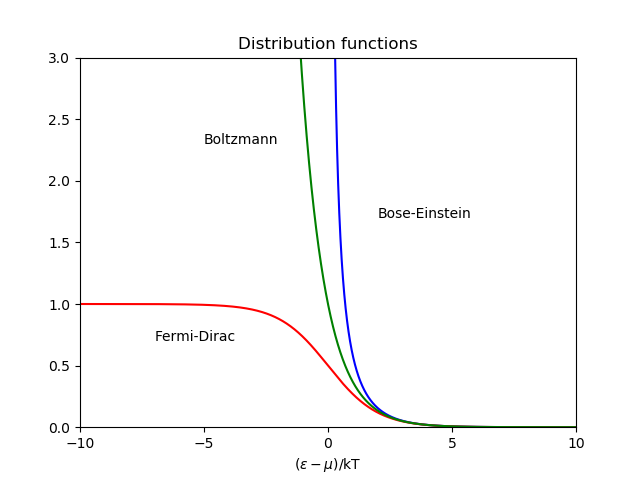
\includegraphics[width=0.7\textwidth]{images/distributions.png}
    \caption{Fermi-Dirac dist. goes to 1 for $\epsilon_{\nu} \gg \mu$}
    \label{fig:dist_therm_stat}
\end{figure} 
s269

In the case of Bose-Einstein: as temperature decreases, $\epsilon - \mu$ goes to zero ($\epsilon$ goes to $\mu$), the distribution diverges. The particles occupy the ground state.

Fermi-Dirac: as T increases towards 0, the distribution becomes a step-function.

Read further page 251 Thermal Physics \cite{ThermalPhysics}
When $\epsilon_{\nu}$ is much greater than $\mu$ the term $\pm 1$ in the denominator of both expressions and they reduce to the Boltzmann distribution. 


\subsection{The ideal Bose gas}

Uniform density: particles in a box with voloum V.
Density inside box: n = N/V

Classical case, use Boltzmann distribution
The termodynamics of an ideal Bose gas is best calculated using the grand canonical ensamble. Then the partition function is 

\begin{equation}
Z(\mu, \beta, V) = \prod_i (1 - \mu e^{(-\beta \epsilon_i)})^{g_i}
\end{equation}

Is This correct?? Check book

Ground state energy

The ideal bose gas is straight forward and have been solved analytically and numerically by many. Weak interacting bosons is also a case that has been studied to a great extent. If we where to add strong interaction the system may do a number of things, flipping of spin, excitation etc.


The ability of bosons at low temperature to collectively inhabit the same energy state, compared to fermions who are restricted to the Pauli exclusion principle.

Free Bose gas - 

\begin{equation} \label{eq:hamilt_free_bose_gas}
H^{free}_V = \int_V dx \frac{1}{2m} \nabla a*(x). \nabla a(x)
\end{equation}


\section{Bose gas in a trap}

As mentioned above, methods for trapping and cooling alkali atom clouds have developed over the last decades, and these systems have been explored considerably. We will now look closet at a Bose gas confined within such a trap and look at the properties of the condensate.
For the BEC the theoretical framework lies within the Gross-Pitaevskii equation, derived by Eugene P. Gross and Lev Petrovich Pitaevskii each in therir own separately papers, 1961.


The Gross-Pitaevskii equation form the basis of studies of dilute Bose gases at zero temperature. It gives the ground-state energy of a system of identical bosons.

Trap: a harmonic oscillator potential trap. 

Consider a dilute Bose gas where the inter-particle distance is much greater than the scattering length. It can be approximated by a mean field theory. We describe it by a simple hard-sphere effective potential. (Master Joachim)

Gross-Pitaevskii - analogy to the Schrödinger equation. 

\subsection{The Gross-Pitaevskii equation}

The time-independent Gross-Pitaevskii equation reads as follows

\begin{equation} \label{Gross-Pitaevskii}
\left( -\frac{\hbar^2}{2m} \frac{\partial^2}{\partial r^2} + V(r) + \frac{4 \pi \hbar^2 a_s}{m}|\psi(r)|^2 \right) \psi(r) = \mu \psi (r)
\end{equation}

For a uniform Bose gas, the GP equation is very simple.

\begin{equation}
\mu = U_0 |\psi (\textbf{r})|^2 = U_0n
\end{equation}

Where $\mu$ being the chemical potential.

page 114
cut-off $k_c$

page 146 equations!

The Bose-Einstein condensation ground state can be described by the Gross-Pitaevskii equation, which uses the Hartree-Fock approximation and the pseduopotential intereaction model. (wiki) 
A a many-body boson system, the Gross-Pitaevskii approach is a mean-field approach. (MBBS)
If the spacing between the particles are greater than the scattering length (in the so-called dilute limit), then one can approximate the true interaction potential that features in this equation by a psedopotential.

READ more about why this is.

Psedopotential: a contact interaction $U_0 \delta(r_i - r_j)$
with $U_0 = \frac{4 \pi \hbar^2 a}{m}$.
We can assume this if the energy is low, zero-temperature, when scattering lenght is much less than the mean interparticle spacing. 
This makes it a mean-field potential. 

The total wave function in the Hartree-Fock approximation of a system of N bosons is represented by the product of single-particle wave functions $\phi$

\begin{equation}
\psi(r_1, r_2, \cdots, r_N) = \phi(r_1) \phi(r_2) \cdots \phi(r_N)
\end{equation}

The pseudopotential model Hamiltonian of the system is given as 

\begin{equation}
H = \sum_{i=1}^N \left( -\frac{\hbar^2}{2m} \frac{\partial^2}{\partial r_i^2} + V(r_i) \right) + \sum_{i<j} \frac{4 \pi \hbar^2 a_s}{m} \delta (r_i - r_j)
\end{equation}

m is the mass of the boson, V is the external potential, $a_s$ is the boson-boson scattering length and $\delta(r)$ the Dirac delta-function. This is an effective potential, the original  with modifications 

The Gross-Pitaevskii equation reads, 

\begin{equation}
\left( -\frac{\hbar^2}{2m} \frac{\partial^2}{\partial r^2} + V(r) + \frac{4 \pi \hbar^2 a_s}{m}|\psi(r)|^2 \right) \psi(r) = \mu \psi (r)
\end{equation}

Se 104 MBBS

Solutions: free particle V(r) = 0

Soliton?

Thomas-Fermi approximation

Bogoliubov approximation: transformation to diagonalize Hamiltionian, yields the stationary solution of the Schrödinger equation. When one must go beyond mean-field theory. 

Interacting Bose gas - Landau's phenomenological theory of superfluidity. Based on the idea that a quantum liquid remains a classical fluid even at zero temperature  and that the classical hydrodynamical laws remain valid. (Many body boson system.) 
Many models have been suggested to create a microscopical theory of the superfluidity. Vortex ring model, hard-sphere model, guassian cluster approach. (wiki)

The properties of these liquids are described in terms of the spectrum of the collective excitations.

\subsection{The wave function}
We are studying a system of two electrons confined in a harmonic oscillator trap described by the Hamiltonian 

\begin{equation}\label{eq:hamilt_trap}
\hat{H} = \sum_{i=1}^N \left( - \frac{1}{2} \nabla_i^2 + \frac{1}{2} \omega^2 r_i^2 \right) + \sum_{i<j} \frac{1}{r_{ij}}
\end{equation}

where the first sum is the standard harmonic oscillator part and the last is the interacting part between the electrons and $N$ represent the number of particles. $\omega$ is the oscillator frequency of the trap and $r_i$ is the position of particle $i$, whereas $r_{ij}$ is the distance between the particles and given as $r_{ij} = |\mathbf{r_i} - \mathbf{r_j}|$. \\

\begin{equation} \label{eq:trap_potential}
 V_{ext}(\mathbf{r}) = 
 \Bigg\{
 \begin{array}{ll}
	 \frac{1}{2}m\omega_{ho}^2r^2 & (S)\\
 \strut
	 \frac{1}{2}m[\omega_{ho}^2(x^2+y^2) + \omega_z^2z^2] & (E)
 \end{array}
\end{equation}

\begin{equation} \label{eq:potential_internal}
 V_{int}(|\mathbf{r}_i-\mathbf{r}_j|) =  \Bigg\{
 \begin{array}{ll}
	 \infty & {|\mathbf{r}_i-\mathbf{r}_j|} \leq {a}\\
	 0 & {|\mathbf{r}_i-_r\mathbf{r}_j|} > {a}
 \end{array}
\end{equation}



\subsection{The ground-state energy}

\section{Strong interacting gases}

At low temperature, liquid helium ($^4$He) becomes a superfluid, but because of strong interactions it is difficult to treat microscopically. In stead one can turn to a hydrodynamical description. Toy model: BEC trests gases, but helium is the only known atom to remain liquid at low temp. 

Thermal physics book, page 168:
Phase shift of Helium-4: at low temp, below 2.2 K it turns to superfluid.
Above this temp. and pressure around 1 bar and up, it is normal liquid. For temp 

\subsection{Liquid $^4$He}
Due to the strong correlation between the atoms in liquid helium, a mean-field approach is inapplicable. Dilute gas, but still interaction plays an important role when temperature is so low. 
The interaction between Helium atoms is strong. Reduces the number of atoms in the zero-momentum state. 
Liquid helium does not solidify at low temperatures. At a threshold it becomes a superfluid, flow through narrow channels without friction. 

Landau: two-fluid description, one part the normal component and another part the superfluid component. 
At normal state the normal component is larger, and the superfluid comp. very small, for liquid helium only 10 percent or lower.
But the fractions are reversed at lower temp. lower then transition temp. 

Elementary excitations: quasiparticles or collective excitations

If quasiparticle is related to fermion, quasiparticle; electron holes (positively charged particles to represent an electron in a valence..)
Collectiv excitations if related to bosons: phonons (particle derived from vibration of atoms in solids) 
Liquid 4-Helium: the energy of dispersion $\epsilon = sp$ s being the velocity of sound and p the momentum.

\subsection{Lennard-Jones potential}


\begin{equation} \label{eq:hamilt_box}
\hat{H} = \sum_{i=1}^N - \frac{1}{2} \nabla_i^2  + \sum_{i<j} V(r)
\end{equation}

\begin{equation} \label{eq:lennard-jones}
V(r) = 4\epsilon \left[ \left( \frac{\sigma}{r} \right)^{12} - \left( \frac{\sigma}{r} \right)^6 \right]
\end{equation}

 
\chapter{Quantum Monte Carlo}
Quantum Monte Carlo is a range of methods that deal with solving the Schrödinger equation by exploiting the statistical features of Monte Carlo simulation in order to handle the multi dimensional integral that rise from the complex quantum many-body problem. As quantum mechanics is a field of statistical nature this is a highly suitable approach and Monte Carlo methods have therefore branched out to a number of different schemes. In this chapter we will focus on one of the most commonly used \textit{Variational Monte Carlo} (VMC) and the more complex \textit{Diffusion Monte Carlo} (DMC).

\section{Variational Monte Carlo}

\cite{hjorthjensen}
page 417-420

page 462

page 537? BEC with Diffusion Monte Carlo

Monte Carlo simulations are widely used methods in numerical science that employs random walkers. 
In this project we are taking a closer look at trapped bosons. We are given a trail wave function we assume is as close to the real case as possible, $\Psi_T(\mathbf{R};\alpha)$ where $\mathbf{R} = (\mathbf{R}_1, ... , \mathbf{R}_N)$ is the position of the different particles. 
From quantum mechanics we know the probability distribution is given by the wave function. 

\begin{equation} \label{eq:prob_dist}
P(\mathbf{R}; \alpha) = \frac{|\Psi_T(\mathbf{R};\alpha)|^2}{\int|\Psi_T(\mathbf{R};\alpha)|^2 d\mathbf{R}}
\end{equation} 

Monte Carlo integration allow us to evaluate the integral at hand. The expectation value of the Hamiltonian is given as follows. 

$$\langle \widehat{\mathbf{H}}\rangle = \frac{\int d \mathbf{R} \Psi^{\ast} (\mathbf{R})H(\mathbf{R}) \Psi(\mathbf{R})}{\int d \mathbf{R} \Psi^{\ast} (\mathbf{R}) \Psi(\mathbf{R})}$$

The variational principle states that the expectation value of the Hamiltonian is an upper-bound for the ground state energy of the Hamiltonian.

$$E_0 \leq \langle H \rangle$$

This is what the Variational Monte Carlo method bases itself on. Given a probability distribution we can evaluate the wave function and look for a local minimum. We define the local energy by

$$\widehat{\mathbf{E}}_L(\mathbf{R};\alpha) = \frac{1}{\Psi_T(\mathbf{R};\alpha)}\widehat{\mathbf{H}}\Psi_T(\mathbf{R};\alpha).$$

Then the expectation value of the local energy is given by

$$\mathbf{E}_V \approx \langle \widehat{\mathbf{E}}_L\rangle = \int P(\mathbf{R}) \widehat{\mathbf{E}}_L d\mathbf{R} \approx \frac{1}{N} \sum_{i = 1}^N \mathbf{E_L}(x_i)$$

where $N$ is the number of Monte Carlo cycles and the points $x_i$ are sampled using the Metropolis-Hastings algorithm. Now we can calculate the probability distribution and the local energy. And for each cycle we propose a new configuration $\mathbf{R}_p$ for the system and hopefully we come closer to the ground state.

$$\mathbf{R}_p = \mathbf{R} + r \ast \Delta \mathbf{R}$$

r is a random number drawn from the distribution $r \in [0, \Lambda]$ with $\Lambda < \infty$, OBS. find out why we choose [0,1] and $\Delta \mathbf{R}$ is the step length of the Metropolis method. Explain some further... 

\cite{toulouse2016introduction}, the advantage of this approach is that it does not use an analytic integration involving the wave function, and thus does not impose severe constraints on the form of the wave function. 
The wave function usually used in QMC are of the Jastrow-Slater form. 

\begin{equation}
\psi(\mathbf{R}) = J(\mathbf{R}) \phi (\mathbf{R})
\end{equation}

Two types of errors are associated with the VMC, the systematic error and  statistical uncertainty. The first error is difficult to know much about, but the latter one however we can calculate. See section on Blocking.

\subsection{Markov chains}
Stochastic process; evolution of a random variable in time. Trajectory of successive points $\mathbf{R}_1, \mathbf{R}_2, ...,\mathbf{R}_N$ with an associated probability distribution $P(\mathbf{R}_N, ...,\mathbf{R}_2,\mathbf{R}_1)$.  

A Markov chain is a stochastic process for which the conditional probability for the transition to a new point $\mathbf{R}_i$ depends only on the previous point $\mathbf{R}_{i-1}$ \cite{toulouse2016introduction}. 

\begin{equation}
P(\mathbf{R}_k|\mathbf{R}_{k-1}, ...,\mathbf{R}_1) = P(\mathbf{R}_k|\mathbf{R}_{k-1})
\end{equation}

We want the walker to be able to move to any configuration within the space that the distribution function spans. So we require that the sampling be \textit{ergodic}. Also we must set another condition on the Markov chain. The condition of \textit{detailed balance}. 

\begin{equation}
P(\mathbf{R}_f|\mathbf{R}_i) \rho(\mathbf{R}_i) = P(\mathbf{R}_i|\mathbf{R}_f) \rho(\mathbf{R}_f)
\end{equation}

This implies the Markov chain be reversible. The probability flux between the two states $\mathbf{R}_i$ and $\mathbf{R}_f$ to be the same in both directions. \cite{toulouse2016introduction}



\subsection{The Metropolis Algorithm}

What is Metropolis algo? Explain some basics...
Given a probability distribution force sampled values to follow this distribution. Employs a stochastic process, a Markov chain.

How we select the new configurations during the simulation is given by the Metropolis Algorithm. 
Ideally we would have a transition probability matrix which told us how likely it would be for each particle to move in the configuration space. Since we don't we try and model it.
We define the following entities:
\\
\\
$P_i^{(n)} \rightarrow$ probability of finding the system in state $i$ at the n'th step.
\\
$j \rightarrow$ possible new step
\\
$A_{i \rightarrow j} \rightarrow$ probability of acceptance. 
\\
$T_{j \rightarrow i} \rightarrow$ probability of making the transition  
\\
\\
Now we can say that a transition probability matrix can be constructed by $T_{j \rightarrow i}A_{j \rightarrow i}.$ The probability of finding the system in state $i$ at step $n$ is

\begin{equation}\label{eq:prob}
P_i^{(n)} = \sum_j \left[P_j^{(n-1)} T_{j \rightarrow i}A_{j \rightarrow i} + P_j^{(n-1)}T_{i \rightarrow j}(1 - A_{i \rightarrow j})\right].
\end{equation}

We want to push the system towards high density regional space of $P_i^{(n)}$. /We want to select states according to the probability distribution. In that way to converge to the desired stationary distribution $p_i$.

$$P_i^{(n \rightarrow \infty)} \rightarrow p_i$$

Using this statement and the fact that the sum over all possible transitional probabilities is one we can rewrite the above equation \ref{eq:prob}.

$$\sum_j [p_j T_{j \rightarrow i}A_{j \rightarrow i} - p_i T_{i \rightarrow j}A_{i \rightarrow j}] = 0$$

In order to stop at the configuration where we have reached equilibrium we us the condition of detailed balance, and it gives us 


$$\frac{A_{j \rightarrow i}}{A_{i \rightarrow j}} = \frac{p_i T_{i \rightarrow j}}{p_j T_{j \rightarrow i}}.$$

We choose to accept when the acceptance is bigger than 1. 

$$A_{j \rightarrow i} = \mathrm{min} \left( 1, \frac{p_i T_{i \rightarrow j}}{p_j T_{j \rightarrow i}}\right)$$

What we must calculate is equation \ref{eq:ratio}. And an example of the code is given further down, in Algorithm \ref{alg:metro}

\begin{equation}\label{eq:ratio}
\frac{p_i T_{i \rightarrow j}}{p_j T_{j \rightarrow i}} = \frac{|\Psi_T(\mathbf{R}_p)|^2}{|\Psi_T(\mathbf{R})|^2}
\end{equation}

\begin{algorithm}
\KwData{matrix $\mathbf{R}$}
\KwResult{float $\mathbf{E}_L$}
number of MC-cycles $N$\;
initialize $\mathbf{R}$\;
calculate $|\Psi_T(\mathbf{R})|^2$\;
\For{i in $[0, N]$}{
    $\mathbf{R}_p = \mathbf{R} + r \ast \Delta \mathbf{R}$\;
    calculate $\omega = \frac{|\Psi_T(\mathbf{R}_p)|^2}{|\Psi_T(\mathbf{R})|^2}$\;
    \eIf{$q \leq \omega$}{
        accept new move\;
    }
    {reject new move\;
    }
    update energy, $\mathbf{E}_L$\;
}
 \caption{Monte Carlo with Metropolis-Hastings}\label{alg:metro}
\end{algorithm}

\subsection{Importance Sampling}

Now we move to an extension of the Metropolis algorithm, the Importance sampling. This method provides us with a better way of suggesting new moves. The expression for the new move, $y$, is given by the solution of the Langevin equation. It reads 

$$y = x + D F(x) \Delta t + \xi \sqrt{\Delta t},$$

where $\xi$ is a gaussian random variable, $D$ is the diffusion coefficient and is $\frac{1}{2}$ and $\Delta t$ is the time step which take values between $[0.001, 0.01]$.
$F(x)$ is the drift force and is given by the gradient of the wave function. 

$$F = 2 \frac{1}{\Psi_T} \nabla \Psi_T$$

It is the drift force that ensures us we move particles towards regions of configuration space where the trail wave function is large. This method increases the efficiency of our program, since the standard Metropolis can suggest new moves in every direction with same probability. 
From the solution of the Fokker-Planck equation we get a new transition probability, the Green's function. 

$$G(y, x, \Delta t) = \frac{1}{(4 \pi D \Delta t)^{3N/2}} \exp (-(y - x - D F(x) \Delta t)^2/4 D \Delta t)$$

Now equation \ref{eq:ratio} from Metropolis algorithm changes to 

$$\frac{p_i T_{i \rightarrow j}}{p_j T_{j \rightarrow i}} = \frac{G(x, y, \Delta t)|\Psi_T(y)|^2}{G(y, x, \Delta t)|\Psi_T(x)|^2},$$

and we must calculate the drift force in order to find new moves and the Green's function to accept/reject these moves.

page 255 in Satistical and thermal physics using Python.

\subsection{Representing the wave function}

Our starting point of the problem at hand is the GP equation \ref{Gross-Pitaevskii}

\begin{equation} \label{eq:trialwf}
 \Psi_T(\mathbf{r})=\Psi_T(\mathbf{r}_1, \mathbf{r}_2, \dots \mathbf{r}_N,\alpha,\beta)=\prod_i g(\alpha,\beta,\mathbf{r}_i)\prod_{i < j}f(a,|\mathbf{r}_i-\mathbf{r}_j|),
\end{equation}

We can incorporate the deformation of the trap in the mean-field wave function. 

\begin{equation} \label{eq:spf_g}
g(\alpha,\beta,\mathbf{r}_i)= \exp{[-\alpha(x_i^2+y_i^2+\beta z_i^2)]}.
\end{equation}

This is the same as 5.10 in \cite{BECCondInDilute}, wave function to describe scattering of two particles...
The ansatz for correlation function, in its simplest form, a Jastrow form:

\begin{equation}
F(1, \cdots, N) = \prod_{i < j}f(a,|\mathbf{r}_i-\mathbf{r}_j|)
\end{equation}

We will use a two-body correlation function that is the solution of the Schrödinger equation of two atoms interaction via a hard-core potential with diameter $a$, at low energy.

\begin{equation} \label{eq:jastrow_f}
    f(a,|\mathbf{r}_i-\mathbf{r}_j|)=\Bigg\{
 \begin{array}{ll}
	 0 & {|\mathbf{r}_i-\mathbf{r}_j|} \leq {a}\\
	 (1-\frac{a}{|\mathbf{r}_i-\mathbf{r}_j|}) & {|\mathbf{r}_i-\mathbf{r}_j|} > {a}.
 \end{array}
\end{equation}

\cite{nilsen2005vortices}, The advantage of using a correlated trial wave function lies in the fact that non-perturbative effects, as the short-range repulsion between atoms may be directly incorporated into the trial wave function.

\section{Gradient Descent}

The variational quantum problem is highly dependent on a good optimization algorithm. One of the more famous and widely used is the gradient descent. It is a family of minimization methods where the idea is to iteratively adjust the parameters in the direction where the gradient of the cost function, usually an energy function, is large and negative \cite{mehta2019high}. 
If a multi-variable function $E(\theta)$ is defined and differentiable in a neighborhood of a point $\theta$, then $E(\theta)$ decreases fastest if one goes from $\theta$ in the direction of the negative gradient of $E$ at $\theta$, $-\nabla E(\theta)$, (wiki). This way we move towards a local minimum in the configurational space. And the gradient descent can be represented as

\begin{equation} \label{eq:theta}
\mathbf{\theta}_{t+1} = \mathbf{\theta}_t - \eta_t \nabla_{\mathbf{\theta}} E(\mathbf{\theta}_t),
\end{equation}

where $\eta_t$ is called the step length/learning rate, it controls how large steps we take within the method.
The easiest way to implement the learning rate is by giving it a constant value. One can however introduce a changing learning rate. This can help us avoid problems like overshooting or oscillating between two points. Such adaptive step size methods can be Newton's method, backtracking line search, Cauchy or Barzilai and Borwein. To be continued. 

We begin by making a guess on the parameter $\theta$, then we follow \eq{theta}. The partial derivative of the energy with respect to the variational parameter can be found through the following equation.

\begin{equation}
\frac{dE_L}{d\alpha} = 2 \left( \left\langle \frac{1}{\Psi_T}\frac{d \Psi_T}{d \alpha} E_L \right\rangle  - \left\langle  \frac{1}{\Psi_T}\frac{d \Psi_T}{d \alpha} \right\rangle \langle E_L \rangle \right)
\end{equation}

Here we will need to calculate the expectation value of the local energy as well as the partial derivative of the wave function, and their product. The term $\frac{1}{\Psi_T}\frac{d \Psi_T}{d \alpha}$ is fairly easy given the wave function we are considering. 

\begin{align} 
\frac{1}{\Psi_T}\frac{d \Psi_T}{d \alpha} &= \frac{-\Psi_T \sum_i^N (x_i^2 + y_i^2 + \beta z^2_i)}{\Psi_T} \\
&= -\sum_i^N (x_i^2 + y_i^2 + \beta z^2_i) \label{eq:frac_deri_wf}
\end{align}

Since the correlation function $f(a, r_{ij})$ of the wave function is independent of the variational parameter $\alpha$, \eq{frac_deri_wf} holds for the interactive case as well.

The last step of the algorithm is to check if the absolute value of the gradient squared is smaller or larger than some given small number $\epsilon$. If larger then we continue the process, if smaller we consider our result good enough. 

\subsection{Stochastic gradient descent}

In this project we are dealing with different types of cost functions. Depending on the method we use the minimization of the first derivative of the cost function is done differently. In the case of linear regression there is no use of numerical optimization methods as there exists an analytical solution to the derivative of the RSS. In the case of logistic regression and the neural network however, there are no closed form solutions to the cost functions being used. We therefore take use of two algorithms called gradient descent and stochastic gradient descent in order to update the parameters (weights).

We call the function we wish to minimize $E(\theta)$, as energy is the quantity we in most problems within physics are trying to minimize. In linear regression this is the MSE (RSS) and in logistic regression it is the cross entropy. 

\begin{equation}
E(\mathbf{\theta}) = \sum_{i=1}^N e_i(X_i, \mathbf{\theta}) 
\end{equation}


In regular gradient descent the algorithm simply updates the parameter $\theta_{t+1}$ according to \eq{theta}. Since the cost function tells us something about how well the parameters work for our regression model we seek to minimize its gradient. Updateing the parameters with \eq{theta} causes the model to moves closer to a local minima. The $\eta$ is called the learning rate and it decides how fast we want to move in the gradients direction. A to large learning rate may cause the model to diverge, but given an optimal value or close to one the gradient descent will converge towards the minima.  

Usually the first parameters are given random variables. 

Gradient descent has some drawbacks, one being that it can get stuck in one local minima and never reaching the correct one. Another is that it is sensitvive to initial conditions, so what values we give the parameters in the begining matters. It is also somewhat computational expensive. A solution to this is stochastic gradient descent.  

\begin{equation}
\nabla_{\theta} E(\theta) = \sum_i^n \nabla_{\theta} e_i(\mathbf{x}_i, \mathbf{\theta}) \longrightarrow \sum_{i \in B_k} \nabla_{\theta} e_i(\mathbf{x}_i, \mathbf{\theta})
\end{equation}

\begin{equation}
\nabla_{\theta} E^{MB} (\theta) = \sum_{i \in B_k}^M \nabla_{\theta} e_i(\mathbf{x}_i, \mathbf{\theta})
\end{equation}

\begin{equation} \label{theta_sgd}
\theta_{t+1} = \mathbf{\theta_t} - \eta_t \nabla_{\theta} E^{MB} (\theta)
\end{equation}

Here we devide the data set into smaller minibatches of size $M$ creating $n/M$ batches. We denote these minibatches $B_k$ running from $k = 1...n/M$. Now we solve the gradient descent for the new minibatches and update the parameters according to \ref{theta_sgd}. Not do we only speed up the computational process, but it also introduces stochasticity. 


\section{Statistical Errors}

When dealing with random variables and estimates we will have to think about how this effect our measurements statistically. Two important properties to evaluate are variance and bias. 

In our case, sampling the probability density $P(\mathbf{R})$ from a sequence of points $\mathbf{R}_i$ through the Metropolis algorithm makes these non-independent (i.e. correlated) as each new sample is selected based on the previous one. See \eq{prob_dist}.

Central limit theorem states that given a sequence of independent and identically distributed random variables drawn from a probability distribution with an expectation value $E[E_L]$, in the limit of number of points N drawn being large, the probability distribution of $E[E_L]$ converges towards a Gaussian (normal) distribution of expected value $E[E_L]$ and variance $V[E_L]/N$.

$\overline{E_L}$ is an estimate of $E_V$ with a statistical uncertainty given by the standard deviation of its Gaussian distribution, 

\begin{equation}
\sigma[\overline{E_L}] = \sqrt{V[\overline{E_L}]}.
\end{equation}

which means that there is a 68.3 \% chance of the expectation value being within the interval [$E_L - \sigma$, $E_L + \sigma$], a 95.5 \% chance of being in the interval [$E_L - 2\sigma$, $E_L + 2\sigma$] and a 99.7 \% chance of being in the interval [$E_L - 3\sigma$, $E_L + 3\sigma$].

However, since we are not dealing with uncorrelated variables, the calculations of the standard deviation is not so straight forward. We will have to make use of some statistical techniques in order to solve the dependencies. We will describe one of the methods in the section on Blocking.

\subsection{Blocking Method}

For the statistical analysis and error estimates we have used the technique of blocking. \
We are looking for the expectation value of the ground state energy of our system. In order to say something about how accurate these results are we want to look at the standard deviation. 

If our samples where uncorrelated we could calculate the standard deviation through the following equation 
$$\sigma = \sqrt{\frac{1}{n - 1} \left(\langle E_L^2\rangle - \langle E_L \rangle^2\right)}.$$

It can be showed that for correlated samples the equation for the standard deviation is
$$\sigma = \sqrt{\frac{1 + 2 \tau / \Delta t}{n - 1} \left(\langle E_L^2\rangle - \langle E_L \rangle^2\right)}$$

where $\tau$ is the time between one sample and the next uncorrelated sample and $\Delta t$ is the time between each sample.\
If we knew what $\tau$ was we could simply find our $\sigma$, but since we don't we use blocking to find it. The method is simple enough, we divide our samples of data into blocks and calculating the mean of each block. So if we have an amount of samples of $\langle E_L \rangle$, we divide these into $M$ blocks and calculate the mean. By plotting the standard deviation as function of the block size we can keep blocking and blocking until we see that the standard deviation stops increasing, and this is where the blocks are uncorrelated. Now we have an estimate for $\tau$ and thus the standard deviation.


\section{Numerical differentiation}
To evaluate the local energy of the system as defined in the project it necessary to compute the second derivative of the trial wave function $\psi_T$. We've chosen to implement the numerical differentiation as a finite difference approximation. Let $\mathbf{R}$ be the row major $N \times D$ matrix where $N$ is the number of particles and $D$ is their dimension. Then the second derivative can be found by the procedure listed as algorithm \ref{alg:nd}

\begin{algorithm}
\KwData{matrix $\mathbf{R}$}
\KwResult{float $\nabla ^2 \psi_T (R)$}
\BlankLine
$\Delta = 0$ \\
$\mathbf{R_p} = \mathbf{R}$\\
$\mathbf{R_m} = \mathbf{R}$\\
\BlankLine
\For{$i$ in $[0, N-1]$}{
	\For{$j$ in $[0, D-1]$}{
		$\mathbf{R_p}(i,j) += h$ \\
		$\mathbf{R_m}(i,j) -= h$ \\
		$\Delta = \psi_T(\mathbf{R_p}) + \psi_T(\mathbf{R_m}) - 2 \psi_T(\mathbf{R})$\\

		$\mathbf{R_p}(i,j) -= h$ \\
		$\mathbf{R_m}(i,j) += h$ \\
	}
}
\KwRet{$\frac{\Delta}{h^2} $}
\BlankLine
\caption{Numerical differentiation of the second order of the trial wave function on a system $\mathbf{R}$}\label{alg:nd}
\end{algorithm} 

Since the derivative involves three function calls for each particle the numerical derivative will obviously be quite computationally expensive. It is noted  that the differentiation could be substantially optimized from the version included in the code, but is outside the scope of this project. 

\section{Diffusion Monte Carlo}

Sources: Lecture notes, Morten \cite{hjorthjensen}

Numerical method solves the many-body Schrödinger equation for the ground-state of a system of boson exactly. Since it does not depend on any a priori choice of wave function. In practice however, one needs a guess of the wave function that is within the range of the exact wave function, or the method would use an enormous amount of time to solve the problem. So in theory DMC can produce the exact ground state of any(?) system, but in practice this is not the case. 

Diffusion Monte Carlo (DMC) is a method within a class of projector Monte Carlo methods. They are methods based on taking projections in Hilbert space. 

\begin{equation}
\exp^{(-\hat{H}t)} \psi(x) = \sum_i c_i \exp^{(-\epsilon_i t)}\phi_i(x) 
\end{equation}

Notes from Jørgens master: Green's function, an ensemble of walkers can be iterated by transitioning between configurations r and r' with probability given the greens function. Rewriting a trail wave function to something looking like a diffusion equation.

Question: what does he mean by the diffusion eq. contributing to the variational method? Is this because of the time-dependent part? Or is this the case for all problems? 




 
\chapter{Machine Learning}
The amount of data in the world today, we need methods to analyse, better and faster. 
Computer science, statistics, mathematics. Methods that can be applied to several branches of science, finance, physics, chemistry, medicine, etc. Important in cosmology, engineering , biophysics 

Suddenly one hears talk of machine learning in many new platforms, radio talk shows, media, the industry is getting more and more interested. Just within the last couple of years machine learning has become a term that people outside of data science and statistical physics known about. 

Sounds like a magical thing, but as we will see during the theory section, some of the most simple statistical methods is reckoned as a method within machine learning.  

What is machine learning? Basically we have some data that we want to analyse, and given a function for measuring the computer is able to find patterns in the data. Depending on what we want is estimate or predict new data. 

Three main groups of machine learning techniques; supervised, unsupervised and reinforcement learning. The lines between this can sometimes be blurred. 

History: 

1952, Arthur Samuel, computer program that could learn as it ran, playing checkers
1958, Frank Rosenblatt designed the first artificial neural network, the Perceptron
1959, Arthur Samuel (wiki), IBM, invented the term machine learning

1960's, book by Nilsson on the topic
1980's, interest in NN started rising again and Hinton Hopfield and Rumelhart, suggested backpropagation 
1982, Hopfield suggested a network with bidirectional lines

1990's, started to flourish as a separate field. 
1997, Deep Blue, chess-playing computer that beat the world chess champion Kasparov
1998, AT\& T Bell Laboratories detecting handwritten postcodes from the US Postal Service.

Have evolved from the field of AI, some ML techniques are closely similated to computer science, some have strong resemblance to classical statistics and deep neural networks developed from the study of human brain. Study of synaptic connections in the brain, with neurons firing off. Simple integrate-and-fire neuron model (or activation functions) to large connected networks.  

Machine learning: how to learn from, and make predictions about, data. \cite{mehta2019high}
Subfield of artificial intelligence. Usually we try to predict than to estimate.

Given some observable quantity $\mathbf{x}$ of the system we wish to study with an related parameter $\mathbf{w}$ of a model $p(\mathbf{x}|\mathbf{w})$ describes the probability of $\mathbf{x}$ given $\mathbf{w}$.
Somehow obtain a dataset $\mathbf{X}$, use these data to fit the model, fitting means, try to find a $\hat{\mathbf{w}}$ using some maximization function, a cost function, to maximize the probability of observing the data. 
$\hat{\mathbf{w}} = \text{argmax}_{\mathbf{w}}{p(\mathbf{X}|\mathbf{w})}$
In case of estimation problems, we want to find the most accurate $\hat{\mathbf{w}}$ where as prediction problems are concerned with the accuracy of the model, $p(\mathbf{x}|\mathbf{w})$, being able to predict new observations. 

Was first explored when studying signal processing in the brain. 
Artificial neuron: each neuron must exceed an activation threshold in order to yield an output, it must be activated. Of the threshold is not made than the neuron remains inactivated, gives zero output.
\begin{equation}
y = f \left( \sum_{i=1}^n w_i x_i \right) = f(u)
\end{equation}

All machine learning techniques require assumptions. In our case it it the wave function. 

\section{Supervised and unsupervised learning}

Dataset $\mathcal{D} =(\mathbf{X}, \mathbf{y})$, and again $\mathbf{X}$ is a matrix of independent variables, $\mathbf{y}$ a vector of the dependent variables. The model $f(\mathbf{x}; \mathbf{\theta})$ is a function that tries to predict an output given the input. And with the cost function $\mathcal{C}(\mathbf{y}, f(\mathbf{X};\mathbf{\theta}))$ we can minimize the error between the predicted output and the true value of the observations $\mathbf{y}$. Fitting the model by minimizing the cost function.

Typically one would use some of the data available to train, $\{\mathbf{X}_{train}, \mathbf{y}_{train}\}$ and some small amount to test the model on.
Then one evaluates the model by testing it on some test data $\mathcal{C}(\mathbf{y}_{test}, f(\{\mathbf{X}_{test}; \theta)\})$



Training set of examples, with a correct response (targets), algorithm generalises to respond correctly to all possible inputs. Called learning from examples.

Supervised learning: discriminative models (classification and regression) 
Must have training data, labeled data, input 
Algorithm is trained from a data set, with a given target


Algorithm generalises, must deal with noise. Overfitting and underfitting, goes for all ML methods. 

unsupervised, algorithm can only exploit similarities in the data to cluster it
Correct response is not given, instead algorithm tries to identify similarities between the input, so inputs with a common characteristics are categorised together. Density estimation.
Dimensionality reduction, clustering

\subsection{Linear Regression}

Can be written, set of data, $(y_i, \mathbf{x}_i)$ where $\mathbf{x}_i$ is the input/the independent variable and $y_i$ is the response. i is the amount of data. 
Lets say we are given a dataset of n samples, $\{ (y_i, \mathbf{x}^{(i)})\}_{i=1}^n$, where $\mathbf{x}^{(i)}$ is the i'th vector of the independent variables, and $y_i$ is the corresponding response. (My words) We wish to find a linear relationship between the independent variable and the response. I.e. the function that describes the response given the data. 

\begin{equation}
y_i = f(\mathbf{X}) = f(\mathbf{x}_i;\mathbf{w}) + \epsilon_i
\end{equation}

Where $\mathbf{X}$ is called the design matrix, $\mathbf{X} \in \mathbb{R}^{n \times p}$, containing all the samples. $\mathbf{w}$ is the parameters we wish to obtain, $\mathbf{w} \in \mathbb{R}^p$, it is the coefficients explicitly describing the function we seek. The column of the design matrix being measured features. $X^{\top} = \{X_0, X_1, X_2, X_3,..., X_p\}$

\begin{equation}
y_i = w_0 + w_1 x_{i1} + w_2 x_{i2} + w_3 x_{i3} + w_4 x_{i4} + ... + w_p x_{ip}
\end{equation}

\begin{equation}
\mathbf{X} = 
\begin{bmatrix}
1 & x_{11} & x_{12} & \dots  & x_{1p} \\
1 & x_{21} & x_{22} & \dots  & x_{2p} \\
\vdots & \vdots & \vdots & \ddots & \vdots \\
1 & x_{n1} & x_{n2} & \dots  & x_{np}
\end{bmatrix}
\end{equation}

This is the matrix we use to solve our problem at hand, and denpending on the matrix having full column rank and the propertie $\mathbf{X^{\top}}\mathbf{X}$ being postive definit we will look at separate methods for finding solutions.

The least square method selects the parameters $w$ so that residual sum of squares (RSS) is minimized.

\begin{equation}
\textnormal{RSS}(w) = \sum_{i=1}^{N} (y_i - x_i^{\top}w)^2
\end{equation}

Searching the minimum of the RSS, we take its derivative wrt. $w$. And we get

\begin{equation}
\hat{w} = (\mathbf{X}^{\top}\mathbf{X})^{-1}\mathbf{X}^{\top}\mathbf{y}
\end{equation}

Hat indicating it is the estimated value. 
This is the expresion we use in the ordinary least square-method in order to find the optimal $w$-values. This method depends on the propertie $\mathbf{X^{\top}}\mathbf{X}$ being postive definit in order to be able to calculate its inverse. In case it is not we must use other method.


\section{Artificial Neural Networks}

Input layer, hidden layers, output layer, uses back propagation
connections, neurons, weights, 
Neural-inspired nonlinear models for supervised learning. 
A supervised learning method. But can also be manipulated to work for unsupervised, ref. to Bendik? 

We can divide neural networks into four categories; general networks for supervised learning, networks designed for image processing, most common one being Convolutional Neural Networks (CNN), networks for sequential data such as Recurrent Neural Networks (RNN) and networks for unsupervised learning such as Deep Boltzmann Machine. 

Multi layered perceptron, a network based on stochastic neuron on thos form, page 369, is known as a boltzmann machine. 

\subsection{Feed-forward Neural Network}

The first and most simplest type of neural network 
9.1.1 i Mehta

\section{Reinforcement learning}

Somewhere in between supervised and unsupervised learning. Algorithm is told when it is wrong but is not told how to correct it. Has to explore and try different possibilities until it works out how to get the answer right. 
Sometimes called learning with a critic, 

page 231 \cite{marsland2014machine}

game theory, game AI, Robot navigation

trail-and-error, a search method, reward and punishment. 

agent-environment-reward, try a state, a reward function evaluates the current solution

Do not have training data
Trained by lowering the Markov chain cost.
Markov chain process, probability distributions, next process depends one the previous

Since we have no data to train the model on, is overfitting an issue in this case? 
Another problem is the complexity of the system, if our trail wave function is not close enough to the exact wave function or can possibly never describe the exact one because it is not complex enough. So we never reach the exact solution. 

read: \cite{mehta2019high}, Mehta on exploration and exploitation


\section{Energy based models}

As mentioned in theory of VMC, many problems in mechanics deal with seeking the energy of a system. Usually the ground state energy. Thermodynamics tells us that every system tries to lower its energy, and this we can take advantage of in energy based models, where we describe the network at hand given an energy model. Typically these types of system have a connecting probability distribution, representing the behavior and characteristics of the system. 

Unlike discriminative models where on tries to perceive differences between data or categories data, energy based models can draw new examples from a probability distribution. Such a method is called a generative model. 

Are closely related to statistical methods, such as Monte Carlo.  \cite{mehta2019high}
Core idea is to produce a probability distribution given the data. From this model we are able to generate new samples. 
Thoughts one generative models: how complex are they to write, and to run (time consuming), how well does the model generalize from training to test and last, which characteristics of the data distribution is the model capable of.
Simple models may not capture structure of a distribution
Complex model may overfit 
Gradient methods for minimizing cost functions
Energy based models do NOT use backpropagation. 
Turn to ideas inspired by MCMC, most common Restricted Boltzmann Machine

Methods where one rewrites the problem to an minimization of energy case. The probability distribution can be the Boltzmann distribution which is dependent on the energy of the system. The energy one tries to minimize. In statistics one deals with observed values $\langle f_i \rangle_{obs}$, which we do not have access to, Instead we replace the observables with empirical averages calculated from data as $\langle f_i \rangle_{data}$ \cite{mehta2019high}.

\subsection{Variational methods}
\cite{mehta2019high}
When dealing with complicated probability distributions, it is often much easier to learn from the relative weights of different states or data points (ratio of probability), than absolute probabilities.  Weights of a Boltzmann distribution are mush easier calculated than the partition function. 
The relative probability of two configurations, $\mathbf{x}_1$ and $\mathbf{x}_2$, are proportional to the difference between their Boltzmann weights.

\begin{equation}
\frac{p(\mathbf{x}_1)}{p(\mathbf{x}_2)} = e^{-\beta (E(\mathbf{x}_1) - E(\mathbf{x}_2))}
\end{equation}

Calculating the absolute probability requires knowledge of the partition function.

\begin{equation}
Z_p = \text{Tr}_{\mathbf{x}} e^{-\beta E(\mathbf{x})}
\end{equation}

Since the probability of the system being in state $\mathbf{x}_1$ is \eqref{eq:prob_boltzmann} dependent on all possible states, i.e. the partition function. 

\begin{equation}
p(\mathbf{x}) = \frac{e^{-\beta E(\mathbf{x}_1)}}{Z_p}
\end{equation}

And calculating it is usually both analytical and numerical difficult.
For example, for the Ising model with N binary spins, the trace involves calculating a sum over $2^n$. In our case we will see that the energy term for the restricted Boltzmann Machine is a three part term where we must sum over both visible nodes as well as all hidden nodes. The number of possible configurations is a very large number, even if we used binary form, if continuous, then it is impossible to calculate over every possible configurations. This is computationally intractable. 

\subsection{Generative model}

\begin{equation}
p(x) = \frac{1}{Z} e^{-\beta (E(x) - \mu N(x))}
\end{equation}

Partition function: estimate it using Monte Carlo (Mean Field Theory) 

Can learn to represent and sample data from a probability distribution.

a model of the conditional probability of the observable X given the target Y. 

Minimizing a cost function using stochastic gradient descent: look closer on this when we describe contrastive divergence. 

\section{Restricted Boltzmann Machine}\label{sec:rbm}

History: restricted Boltzmann Machine was developed by Geoffrey Hinton, at the University of Toronto and Google. Read more.

\subsection{The Network}

RBM is a bipartite graph, which means that the nodes in each layer can be dealt with separately. We can use CD, see section below. 
We can think of RBM as a two-layer neural network, with one visible and one hidden layer. This is similar to feed-forward neural network  with logistic activation (assuming hidden nodes are binary). Training is different, CD with Markov chain. Refer to section on artificial neural network

Restricted Boltzmann machine is a energy-based generative model which include hidden and visible variables (ref to Metha). It consists of a two-layer network with a two dimensional matrix $W_{ij}$ telling how strong the connections between the hidden and visible nodes are. The energy related to a configuration of the nodes is what forms the basis of our model. It is given in \eqref{eq:E_rbm}.

\subsection{The energy function}
\begin{equation}\label{eq:E_rbm}
E(\mathbf{v}, \mathbf{h}) = - \sum_{i} a_i(v_i) - \sum_{\mu} b_j(h_j) - \sum_{ij} W_{ij}v_i h_j 
\end{equation}

Here $a_i(v_i)$ and $b_j(h_j)$ are bias functions of the visible and hidden layers which we are allowed to choose our self. In our case we want the visible layer to take a continuous form and the hidden layer to be binary, (Gaussian-binary), meaning $a_i$ and $b_j$ takes the following from

$$a_i(v_i) = \frac{v_i^2}{2 \sigma_i^2}, \ \ \ b_j(h_j)= b_jh_j.$$

We are working with restricted Boltzmann machine meaning there is no connection between nodes within layers, only between layers. Also this network is a generative one so we want our network to learn a probability distribution. We begin with the joint probability distribution of the visible and hidden nodes is given in \eqref{eq:F_rbm_joint} where $Z$ is the partition function, see \eqref{eq:Z}. 

\begin{equation}\label{eq:F_rbm_joint}
F_{rbm} (\mathbf{X}, \mathbf{h}) = \frac{1}{Z} e^{-E(\mathbf{X}, \mathbf{h})}
\end{equation}

\begin{equation}\label{eq:Z}
Z = \int \int \frac{1}{Z} e^{-E(\mathbf{X}, \mathbf{h})} d\mathbf{x}d\mathbf{h}
\end{equation}

From \eqref{eq:F_rbm_joint} we can marginalize over all the hidden units and get the distribution over the visible units. And as mentioned above this is what we use to represent our wave function. 

\begin{align}\label{eq:F_rbm_marg}
F_{rbm} (\mathbf{X}) &= \sum_{\mathbf{h}} F_{rbm} (\mathbf{X}, \mathbf{h}) \\
&= \frac{1}{Z} \sum_{\mathbf{h}} e^{-E(\mathbf{X}, \mathbf{h})}
\end{align}

Since we have no data to train we use the technique of reinforcement learning. We feed the network with input using Monte Carlo method and based on the variational principle we find the ground state of the system by seeking the configuration that gives the lowest quantum mechanical energy. According to this principle we change the weights and biases by gradient descent method and hopefully the network will converge towards the correct state.  

Because of the symmetric connection in a regular Boltzmann machine, it is actually a Markov Random Field. section 16.2 in book. 
It is computational expensive because all nodes are dependent on one another. 
So we turn to restricted Boltzmann Machine, all nodes in each layer is independent of each other. By treating each hidden neuron as an individual 'expert' and multiplying together their distribution for each visible neuron it is possible to compute the probability distribution for each visible neuron. And visa versa one finds the distribution over the hidden nodes by computing over the visible nodes. 

The visible nodes are clamped during 'awake' training. 
Algorithm used is called Contrastive Divergence (CD)

\subsection{Representing the wave function}

Our wave function is given from the energy of the restricted Boltzmann machine, see \eqref{eq:E_rbm}, which is the joint energy functional between the visible and hidden nodes. From the marginal probability of the joint probability distribution, see \eqref{eq:F_rbm_marg}, we get our wave equation.                     

\begin{align}\label{eq:F_rbm}
\Psi(X) &= F_{rbm}(X) \\
&= \frac{1}{Z} \exp \left( -\sum_{i}^{M} \frac{(X_i - a_i)^2}{2 \sigma^2} \right) \prod_{j}^{N} \left( 1 + \exp \left( b_j + \sum_{i}^{M} \frac{X_i \omega_{ij}}{\sigma^2} \right) \right)
\end{align}

Here $Z$ is the partition function, $X_i$ represents the visible nodes running up to $M$, and $a_i$ and $b_j$ are the biases described in the section below, \eqref{sec:rbm}, where number of hidden nodes $j$ runs up to $N$. 

$\omega_{ij}$ is an $M \times N$ matrix holding the weights connecting the visible nodes with the hidden and $\sigma$ is the standard deviation of the noise in our model. \\


\section{Gibbs Sampling}

\subsection{Maximum Likelihood}

Cost function: 
In Maximum Likelihood estimation (MLE), maximize the log likelihood of the training data.
Maximize the probability of the data (generating the observed data).

Log likelihood based on $N$ training inputs, 

\begin{align}
\mathcal{L} &= \frac{1}{N} \sum_{n=1}^N \log p(\mathbf{x}^n, \mathbf{W}) \\
&= \langle \log p(\mathbf{x}, \mathbf{W}) \rangle \\
&= -\frac{1}{2} \langle (\mathbf{x}^n)^T \mathbf{W} \mathbf{x}^n \rangle_{\text{data}} - \log Z(\mathbf{W}) \\
&= E_{\mathbf{h} \sim P(\mathbf{h}|\mathbf{v_n};W)}[\mathbf{v}_n^T \mathbf{h}] - E_{\mathbf{v}, \mathbf{h} \sim P(\mathbf{v},\mathbf{h};W)}[\mathbf{v}^T \mathbf{h}] \\
=& \text{data term} - \text{model term}
\end{align}

Used the fact that our generative model takes a Boltzmann form and that the partition function is independent of the data. Now that we have our cost function we need a way to minimize it, one way is to use stochastic gradient descent. As we know from theory above, for this method we must have the gradient of log-likelihood to minimize. This must be derived with respect to the parameter the energy function is based on. 

\subsection{Contrastive Divergence}


In most cases the expectation value with respect to the model is difficult to compute, since it involves the partition function, which we mentioned is impossible to compute.
We therefore approximate it using Gibbs samling. 

\begin{equation}
\frac{\partial \mathcal{L}}{\partial \mathbf{W}} = - \langle \frac{\partial \mathcal{L}}{\partial \mathbf{W}} \rangle_{\text{data}} + \langle \frac{\partial \mathcal{L}}{\partial \mathbf{W}} \rangle_{p(\mathbf{x}, \mathbf{W})}
\end{equation}

An alternative view on maximizing the log-likelihood is minimizing the difference between the two probability distributions, the one given the data and the one produced by the model. 
What Hinton suggested was that instead of minimizing the difference between two probabilities, where one is expensive to compute, one minimizes the difference between the 
This is sometimes in literature called a fantasy particle, which we produce with MCMC. 

\subsection{Cost function}

Here is where we deviate from what is common in machine learning, instead of a cost function based on some dataset, our cost function is the energy of the quantum mechanical system. Like in gradient descent, we use the function, \eqref{eq:energy_gradient}. 
But now we must take in to account that we have four variational parameters instead of the one before, in VMC. So the first derivative of the wave function  

\subsection{Algorithm}

\cite{marsland2014machine}

A Markov Chain Monte Carlo method for sampling expectation values. This is possible because the visible units and the hidden units are conditionally independent (restricted boltzmann machine). We sample from the joint distribution. 

\begin{equation}
p(\mathbf{v}|\mathbf{h}) = \prod_i p(v_i|\mathbf{h})
\end{equation}

\begin{equation}
p(\mathbf{h}|\mathbf{v}) = \prod_j p(h_j|\mathbf{v})
\end{equation}

The idea of Gibbs is to iteratively sample from the conditional distributions $\mathbf{h}_{t+1} \sim p(\mathbf{h}|\mathbf{v}_t)$ and $\mathbf{v}_{t+1} \sim p(\mathbf{v}|\mathbf{h}_{t+1})$. At the end of the Gibbs sampling one ends up with a minibatch of samples, the so called fantasy particles mentioned before. But instead of doing $N$ such iterations/samples which would take a lot of time, we draw one time and then use this configuration and work the RBM. This is basically the Contrastive Divergence method. 

We represent the wave equation on a new form. This requires that the wave function is positive definite. 

\begin{equation}\label{eq:Gibbs}
\psi(x) = \sqrt{(F_{rbm})}
\end{equation}

Rather than on the form we have used before.

\begin{equation}\label{eq:Gibbs_new}
\psi(x) = (F_{rbm})
\end{equation}

Conditional probability density functions: 
conditional probability of a binary hidden unit $h_j$ being on or off takes the form of a sigmoid function:

\begin{equation}
p_{GB}(h_j = 1|\mathbf{x}) = \frac{1}{1 + e^{-b_j - (\frac{x}{\sigma^2})^T \mathbf{w}_{*j} }}
\end{equation}

The conditional probability of continuous $\mathbf{x}$ has another form,
\begin{equation}
p_{GB}(x_i = 1|\mathbf{h}) = \mathcal{N}(x_i|b_i +  \mathbf{w}^T_{i*}, \sigma^2_i)
\end{equation}


\begin{itemize}
    \item Gibbs sampling 
\begin{itemize}
    \item Initialize $\mathbf{v}$
    \item Sampling $\mathbf{h}$ with $P(\mathbf{h}|\mathbf{v})$
    \item Sampling $\mathbf{v}$ with $P(\mathbf{v}|\mathbf{h})$
    \item Iterate step 2 and 3
\end{itemize}
\end{itemize}

\part{Implementation and results}

\chapter{Implementation}
The interaction term $V_{int}$ we can leave out of the VMC sampler class, since the trail wave equation will guarantee that the particles do not move to close to each other. Meaning not closer than the boundary $a$, in which the wave equation becomes zero. So we simply leave this out of the computations in order to move unnecessary calculations. 
Or it may be excluded given the sampling method assures we do not select a new suggested position with a probability lower than some random number $\epsilon$.  

\chapter{Results}
Properties to calculate:

energy, mean radial displacement, one-body density, two-body density, learning rate, standard deviation, variation, for RBM, plot the matrix W.
Confidence interval 

Notes results(draft)

All for 2 particles in 3 dimensions.

Biggest Problem!! $\alpha$ will NOT stabilise, only increases when interaction is on....  
And method fluctuates too much, energy does not stabilises. Gradient of local energy is to high, solution? 
Problem with energy being both too high AND too low..

\section{Non-interacting}
Used the analytic solution of the local energy
\subsection{Metropolis}
Run with naive metropolis works fine. 
Monte Carlo cycles = $10^5$


\subsection{Importance}
Run with numerical calculation of the quantum force $F$ is ok, number of Monte Carlo cycles = $10^5$

Energy stabilises after few gradient descent runs, 100 something runs. 

Optimal $\alpha$ is also reached

Importance sampling with analytical solution to the quantum force also works fine. 

Monte Carlo cycles = $10^5$

\section{Weak interacting}
Used the analytic AND numerical solution of the local energy

With a = 0.00433, correct total energy = 3.00345

a = 0.433, total energy = 3.3827
\subsection{Metropolis}
With numerical calculation of the local energy:

Not correct energy

Total energy = 2.998 ish and alpha approx 0.5006

With analytical calculation of the local energy:

Total energy = 2.998 ish and alpha approx 0.5006
But the derivative of the energy is high! So something is wrong with the gradient method??

\subsection{Importance}
Monte Carlo cycles = $10^5$
With numerical calculation of the local energy:

- and numerical solution of quantum force

Not correct energy nor alpha

Energy stabilises at to low, 2.998 and alpha is to high, above 0.5006
 
- analytical solution of quantum force
With my own expression the method does not work at all, energy and alpha waaay to high..
Used Håkons expression of the factor i derivative of $u$, times 2. Do NOT know why this worked. Must find that out.. 

Still not correct energy though, but closer to the correct one. Alpha still to high

Energy goes too high, 3.005 and alpha is to high, approx 0.5033

With analytical calculation of the local energy:

- and numerical solution of quantum force

Energy around 3.011, alpha 0.50326, not entirely correct...
 
- analytical solution of quantum force

Energy around 3.01, alpha 0.50326, not entirely correct...

\section{Strong interaction}
\subsection{Metropolis}


\subsection{Importance}


\subsection{Gibbs}
 
\chapter{Conclusion}
\input{chapters/conclusion}

\appendix
\chapter{Appendix Title}
\section{Derivations}
\subsection{Local energy}\label{app:el}

\setlength\parindent{0pt}

The local energy is given by

$$E_L(\mathbf{r})=\frac{1}{\Psi_T(\mathbf{r})}\hat{H}\Psi_T(\mathbf{r})$$

with trial wave equation

$$\Psi_T(\mathbf{r}) = \prod_{i} g(\alpha, \beta, \mathbf{r_i}) \prod_{i<j} f(a, |\mathbf{r_i} - \mathbf{r_j}|)$$

The Hamiltonian becomes

$$\hat{H} = \sum_{i}^{N} \left( \frac{-\hbar^2}{2m} \nabla_i^2 + V_{ext}(\mathbf{r_i})\right) + \sum_{i>j}^{N} V_{int}(\mathbf{r_i}, \mathbf{r_j})$$

where  

$$
V_{ext}(\mathbf{r_i}) = 
\begin{cases}
\frac{1}{2} m\omega_{ho}^2 r^2\ \ \ \ \ \ \ \ \ \ \ \ \ \ \ \ \ \ \ \ \ \ \ \ (S)\\
\frac{1}{2} m [\omega_{ho}^2(x^2+ y^2) + \omega_z^2 z^2]\ \ \  (E)
\end{cases}
$$

and

$$
V_{int}(|\mathbf{r_i} - \mathbf{r_j}|) = 
\begin{cases}
\infty \ \ \ \   |\mathbf{r_i} - \mathbf{r_j}| \le a \\
0 \ \ \ \ \ \ |\mathbf{r_i} - \mathbf{r_j}| > a
\end{cases}
$$


First we solve only the harmonic oscillator (a=0) and we use $\beta = 1$ for one particle in 1D.

And for one particle the trial wave equation, Hamiltonian and local energy becomes

\begin{align}
\Psi_T(\mathbf{r}) &= g(\alpha, x) = e^{-\alpha x_i^2}, \\
\hat{H} &= \left( \frac{-\hbar^2}{2m} \nabla^2 + \frac{1}{2} m\omega_{ho}^2 x^2\right) \\
E_L &= \frac{1}{e^{-\alpha x^2}}\left( \frac{-\hbar^2}{2m} \nabla^2 (e^{-\alpha x^2}) + \frac{1}{2} m\omega_{ho}^2 x^2(e^{-\alpha x^2})\right)
\end{align}
We then need  to compute the laplacian of the trial wave-function. 
\begin{align}
\nabla^2(e^{-\alpha x^2}) &= \frac{d^2 e^{-\alpha x^2}}{dx^2}\\
&= \frac{d}{dx} \left(\frac{de^{-\alpha x^2}}{dx}\right)\\
&= \frac{d}{dx} (-2\alpha x \cdot e^{-\alpha x^2})\\
&= (4\alpha^2 x^2 - 2\alpha)e^{-\alpha x^2} 
\end{align}
Finally, the local energy becomes 

\begin{align}
E_L &= \frac{e^{-\alpha x^2}}{e^{-\alpha x^2}}\left( \frac{-\hbar^2}{2m}  (4\alpha^2 x^2 - 2\alpha) + \frac{1}{2} m\omega_{ho}^2 x^2\right) \\
E_L &= \frac{-\hbar^2}{2m}(4\alpha^2 x^2 - 2\alpha) + \frac{1}{2} m\omega_{ho}^2 x^2
\end{align}
Solving the same problem for one particle in 2D and 3D we get something similar, 

\begin{align}
E_L &= (\frac{-\hbar^2}{2m})4\alpha^2 (x^2 + y^2) - 4\alpha + \frac{1}{2} m\omega_{ho}^2 (x^2 + y^2),\\
E_L &= (\frac{-\hbar^2}{2m})4\alpha^2 (x^2 + y^2 + z^2) - 6\alpha + \frac{1}{2} m\omega_{ho}^2 (x^2 + y^2 + z^2)
\end{align}
We can now easily see that the local energy energy for N number of particles in 1D, 2D and 3D becomes

\begin{equation}\label{eq:el_ni}
\begin{split}
\text{1D: }E_L &= \sum_i^N (\frac{-\hbar^2}{2m})[4\alpha^2 (x^2) - 2\alpha] + \frac{1}{2} m\omega_{ho}^2 (x^2),\\
\text{2D: }E_L &= \sum_i^N (\frac{-\hbar^2}{2m})[4\alpha^2 (x^2 + y^2) - 4\alpha] + \frac{1}{2} m\omega_{ho}^2 (x^2 + y^2)\\
\text{3D: }E_L &= \sum_i^N (\frac{-\hbar^2}{2m})[4\alpha^2 (x^2 + y^2 + \beta^2 z^2) - 4\alpha -2\alpha \beta] + \frac{1}{2} m\omega_{ho}^2 (x^2 + y^2 + \beta z^2)
\end{split}
\end{equation}

since the energy is simply the sum of the derivatives of each particle.

Now we can try to solve the complete problem. The trial wave function is now

$$\Psi_T(\mathbf{r}) = \prod_{i} g(\alpha, \beta, \mathbf{r_i}) \prod_{i<j} f(a, |\mathbf{r_i} - \mathbf{r_j}|)$$

and first we rewrite it using 

$$g(\alpha, \beta, \mathbf{r_i}) = \exp -\alpha (x_i^2 + y_i^2 + \beta z_i^2) = \phi (\mathbf{r_i})$$

and 

$$f(r_{ij})\exp \left(\sum_{i<j}u(r_{ij})\right)$$

getting 

$$\Psi_T(\mathbf{r}) = \prod_{i} \phi (r_i) \exp \left(\sum_{i<j}u(r_{ij})\right).$$

The local energy for this problem becomes:


\begin{equation} \label{eq:local energy}
E_L = \frac{1}{\Psi_T(\boldsymbol{r})} \left( \sum_{i}^{N} \left(\frac{\hbar^2}{2m} \nabla_i^2 \Psi_T(\mathbf{r}) + \frac{1}{2} m\omega_{ho}^2 r^2 \Psi_T(\mathbf{r}) \right) + \sum_{i<j}^{N} V_{int}(\mathbf{r_i},\mathbf{r_j}) \Psi_T(\mathbf{r}) \right).
\end{equation}

The difficulty in \eqref{eq:local energy} is solving the derivatives of the wave equation given the complexity of the exponential. We begin with the first derivative.

$$\nabla_i^2 \prod_{i} \phi (\mathbf{r_i}) \exp \left(\sum_{i<j}u(r_{ij})\right) = \nabla_i \cdot \nabla_i \prod_{i} \phi (\mathbf{r_i}) \exp \left(\sum_{i<j}u(r_{ij})\right)$$

The first derivative of particle k:

$$\nabla_k \prod_{i} \phi (\mathbf{r_i}) \exp \left(\sum_{i<j}u(r_{ij})\right) = \nabla_k \left( \prod_{i} \phi (\mathbf{r_i}) \right) \exp \left(\sum_{i<j}u(r_{ij})\right) + \nabla_k \left(\exp \left(\sum_{i<j}u(r_{ij})\right)\right)  \prod_{i} \phi (r_i) $$

\begin{align*}
\nabla_k \left( \prod_{i} \phi (\mathbf{r_i}) \right) &= \nabla_k (\phi(r_1)(\phi(r_2)...(\phi(r_k)..(\phi(r_N)) \\
&=\nabla_k \left(e^{-\alpha (x_1^2 + y_1^2 + z_1^2)} e^{-\alpha (x_2^2 + y_2^2 + z_2^2)} ... e^{-\alpha (x_k^2 + y_k^2 + z_k^2)} ... e^{-\alpha (x_N^2 + y_N^2 + z_N^2)}\right)\\
&=\nabla_k \phi(r_k) \left[\prod_{i\ne k} \phi(\mathbf{r_i})\right]\\
\nabla_k \exp \left(\sum_{i<j}u(r_{ij})\right) &= \nabla_k \exp (u(r_{12}) + u(r_{13}) + ... + u(r_{23}) + ... + u(r_{kj}) + .. + u(r_{N-1,N}) )\\
&=\exp \left(\sum_{i<j}u(r_{ij})\right) \sum_{i\ne k} \nabla_k u(r_{kj})
\end{align*}

And the first derivative of the trial wave equation is

$$\nabla_k \Psi_T(\mathbf{r}) = \nabla_k \phi(r_k) \left[\prod_{i\ne k} \phi(\mathbf{r_i})\right] \exp \left(\sum_{i<j}u(r_{ij})\right) +  \prod_{i} \phi (\mathbf{r_i}) \exp \left(\sum_{i<j}u(r_{ij})\right) \sum_{j\ne k} \nabla_k u(r_{kj}).$$

Now we find the second derivative of the wave function.

\begin{align*}
\frac{1}{\Psi_T(\mathbf{r})}\nabla_k^2 \Psi_T(\mathbf{r}) &= \frac{1}{\nabla_k \prod_{i} \phi (\mathbf{r_i}) \exp \left(\sum_{i<j}u(r_{ij})\right)} \left( \nabla_k \left( \nabla_k \phi(r_k) \left[\prod_{i\ne k} \phi(\mathbf{r_i})\right] \right) \cdot \exp \left(\sum_{i<j}u(r_{ij})\right)  \right. \\
\\
&+\nabla_k \phi(r_k) \left[\prod_{i\ne k} \phi(\mathbf{r_i})\right] \cdot \nabla_k \left( \exp \left(\sum_{i<j}u(r_{ij})\right)\right)\\
\\
&+\nabla_k \left( \prod_{i} \phi (\mathbf{r_i}) \right) \cdot \exp \left(\sum_{i<j}u(r_{ij})\right) \sum_{j\ne k} \nabla_k u(r_{kj}) \\
\\
&+ \prod_{i} \phi (\mathbf{r_i}) \cdot \nabla_k \left(\exp \left(\sum_{i<j}u(r_{ij})\right)\right) \sum_{j\ne k} \nabla_k u(r_{kj})  \\
\\
&+ \left. \prod_{i} \phi (\mathbf{r_i}) \exp \left(\sum_{i<j}u(r_{ij})\right) \cdot \nabla_k \left(\sum_{j\ne k} \nabla_k u(r_{kj}) \right) \right) \\
\end{align*}

Solving these equations separately makes it easier.

$$\frac{\nabla_k^2 \phi(r_k) \left[\prod_{i\ne k} \phi(\mathbf{r_i})\right]  \cdot \exp \left(\sum_{i<j}u(r_{ij})\right)}{\nabla_k \prod_{i} \phi (\mathbf{r_i}) \exp \left(\sum_{i<j}u(r_{ij})\right)} = \frac{\nabla_k^2 \phi(r_k)}{\phi(r_k)}$$

$$\frac{\nabla_k \phi(r_k) \left[\prod_{i\ne k} \phi(\mathbf{r_i})\right] \cdot \nabla_k \left( \exp \left(\sum_{i<j}u(r_{ij})\right)\right)}{\nabla_k \prod_{i} \phi (\mathbf{r_i}) \exp \left(\sum_{i<j}u(r_{ij})\right)} = \frac{\nabla_k \phi(r_k)}{\phi(r_k)} \sum_{j \ne k} \nabla_k u(r_{kj})$$

$$\frac{\nabla_k \left( \prod_{i} \phi (\mathbf{r_i}) \right) \cdot \exp \left(\sum_{i<j}u(r_{ij})\right) \sum_{j\ne k} \nabla_k u(r_{kj})}{\nabla_k \prod_{i} \phi (\mathbf{r_i}) \exp \left(\sum_{i<j}u(r_{ij})\right)} = \frac{\nabla_k \phi(r_k)}{\phi(r_k)} \sum_{j \ne k} \nabla_k u(r_{kj})$$

$$\frac{\prod_{i} \phi (\mathbf{r_i}) \cdot \nabla_k \left(\exp \left(\sum_{i<j}u(r_{ij})\right)\right) \sum_{j\ne k} \nabla_k u(r_{kj})}{\nabla_k \prod_{i} \phi (\mathbf{r_i}) \exp \left(\sum_{i<j}u(r_{ij})\right)} =  \sum_{i \ne k} \nabla_k u(r_{ki}) \sum_{j \ne k} \nabla_k u(r_{kj})$$

$$\frac{\prod_{i} \phi (\mathbf{r_i}) \exp \left(\sum_{i<j}u(r_{ij})\right) \cdot \nabla_k \left(\sum_{j\ne k} \nabla_k u(r_{kj}) \right)}{\nabla_k \prod_{i} \phi (\mathbf{r_i}) \exp \left(\sum_{i<j}u(r_{ij})\right)} = \sum_{j \ne k} \nabla_k^2 u(r_{kj})$$

Putting them together again we get the following

\begin{equation} \label{eq:local energy 2}
\frac{1}{\Psi_T(\mathbf{r})}\nabla_k^2 \Psi_T(\mathbf{r}) = \frac{\nabla_k^2 \phi(r_k)}{\phi(r_k)} + 2\frac{\nabla_k \phi(r_k)}{\phi(r_k)} \sum_{j \ne k} \nabla_k u(r_{kj}) + \sum_{i \ne k} \nabla_k u(r_{ki}) \sum_{j \ne k} \nabla_k u(r_{kj}) + \sum_{j \ne k} \nabla_k^2 u(r_{kj})
\end{equation}


We solve the first and second derivatives of $u(r_{kj})$.

\begin{equation} \label{first der}
\nabla_k u(r_{kj}) = \left(\vec{i} \frac{\partial}{\partial x_k} + \vec{j} \frac{\partial}{\partial y_k} + \vec{k} \frac{\partial}{\partial z_k}\right) u(r_{kj})
\end{equation}

From Rottmann p. 128 we have that

\begin{align*}
\frac{\partial u(r_{kj})}{\partial x_k}\ \vec{i}  &= \frac{\partial u(r_{kj})}{\partial r_{kj}} \frac{\partial r_{kj}}{\partial x_k} \ \vec{i}\\
&= u'(r_{kj}) \frac{\partial \sqrt{|x_k - x_j|^2 + |y_k - y_j|^2 + |z_k - z_j|^2}}{\partial x_k} \vec{i}\\
&=u'(r_{kj}) \frac{1}{2} 2 |x_k - x_j|\frac{1}{r_{kj}} \vec{i}\\
&=\frac{u'(r_{kj})|x_k - x_j|}{r_{kj}} \vec{i}\\
\frac{\partial u(r_{kj})}{\partial y_k}\ \vec{j}  &= \frac{u'(r_{kj})|y_k - y_j|}{r_{kj}} \vec{j}\\
\frac{\partial u(r_{kj})}{\partial z_k}\ \vec{k}  &=\frac{u'(r_{kj})|z_k - z_j|}{r_{kj}} \vec{k}
\end{align*}

where we have used the fact that $r_{kj} = \sqrt{|x_k - x_j|^2 + |y_k - y_j|^2 + |z_k - z_j|^2}$. Now equation \eqref{first der} becomes

\begin{align*}
\nabla_k u(r_{kj}) &= u'(r_{kj})\frac{(|x_k - x_j|\vec{i} + |y_k - y_j|\vec{j} + |z_k - z_j|\vec{k})}{r_{kj}}\\
&= u'(r_{kj}) \frac{(\boldsymbol{r_k} - \boldsymbol{r_j})}{r_{kj}}.
\end{align*}

And for the second derivative have that

\begin{equation} \label{second der}
\nabla_k^2 u(r_{kj}) = \left(\frac{\partial^2}{\partial x_k^2} + \frac{\partial^2}{\partial y_k^2} + \frac{\partial^2}{\partial z_k^2}\right) u(r_{kj})
\end{equation}

and use Rottmann p. 128 again and see that

\begin{align*}
\frac{\partial^2 u(r_{kj})}{\partial x_{kj}^2} &= \frac{\partial^2 u(r_{kj})}{\partial r_{kj}^2} \left(\frac{\partial r_{kj}}{\partial x_{kj}}\right)^2 + \frac{\partial u(r_{kj})}{\partial r_{kj}} \frac{\partial^2 r_{kj}}{\partial x_{kj}^2}\\
& =u''(r_{kj}) \frac{(x_k - x_j)^2}{r_{kj}^2} + u'(r_{kj}) \frac{\partial^2 r_{kj}}{\partial x_{kj}^2}\\
\frac{\partial^2 r_{kj}}{\partial x_{kj}^2} &= \frac{\partial^2 \sqrt{|x_k - x_j|^2 + |y_k - y_j|^2 + |z_k - z_j|^2}}{\partial x_{kj}^2}\\
&= \frac{\partial \frac{x_k - x_j}{\sqrt{|x_k - x_j|^2 + |y_k - y_j|^2 + |z_k - z_j|^2}}}{\partial x_{kj}}\\
&= \frac{r_{kj} - \frac{1}{2} (x_k - x_j) \cdot \frac{2(x_k - x_j)}{r_{kj}}}{r_{kj}^2}\\
&= \frac{1}{r_{kj}} - \frac{(x_k - x_j)^2}{r_{kj}^3}.
\end{align*}

These equations put together and solving with respect to $y$ and $z$ we get 

\begin{align*}
\frac{\partial^2 u(r_{kj})}{\partial x_{kj}^2} &= u''(r_{kj}) \frac{(x_k - x_j)^2}{r_{kj}^2} + u'(r_{kj}) \left(\frac{1}{r_{kj}} - \frac{(x_k - x_j)^2}{r_{kj}^3}\right),\\
\frac{\partial^2 u(r_{kj})}{\partial y_{kj}^2} &= u''(r_{kj}) \frac{(y_k - y_j)^2}{r_{kj}^2} + u'(r_{kj}) \left(\frac{1}{r_{kj}} - \frac{(y_k - y_j)^2}{r_{kj}^3}\right),\\
\frac{\partial^2 u(r_{kj})}{\partial z_{kj}^2} &= u''(r_{kj}) \frac{(z_k - z_j)^2}{r_{kj}^2} + u'(r_{kj}) \left(\frac{1}{r_{kj}} - \frac{(z_k - z_j)^2}{r_{kj}^3}\right).
\end{align*}

Now we can add them all together and equation \eqref{second der} becomes

\begin{align*}
\nabla_k^2 u(r_{kj}) &= \frac{u''(r_{kj})}{r_{kj}^2} ((x_k - x_j)^2 + (y_k - y_j)^2 + (z_k - z_j)^2) \\
&+ u'(r_{kj}) \left(\frac{3}{r_{kj}} - \frac{(x_k - x_j)^2 + (y_k - y_j)^2 + (z_k - z_j)^2}{r_{kj}^3}\right)\\
&= \frac{u''(r_{kj}) r_{kj}^2}{r_{kj}^2} + u'(r_{kj}) \left( \frac{3}{r_{kj}} - \frac{r_{kj}^2}{r_{kj}^3}\right)\\
&= u''(r_{kj}) + u'(r_{kj})\frac{2}{r_{kj}}
\end{align*}

Now we can write out the complete second derivative, equation \eqref{eq:local energy 2} 

\begin{align*}
\frac{1}{\Psi_T(\mathbf{r})}\nabla_k^2 \Psi_T(\mathbf{r}) &= \frac{\nabla_k^2 \phi(r_k)}{\phi(r_k)} + 2\frac{\nabla_k \phi(r_k)}{\phi(r_k)} \sum_{j \ne k} \frac{(\boldsymbol{r_k} - \boldsymbol{r_j})}{r_{kj}} u'(r_{kj}) \\
&+ \sum_{ij \ne k} \frac{(\boldsymbol{r_k} - \boldsymbol{r_i})}{r_{ki}} \frac{(\boldsymbol{r_k} - \boldsymbol{r_j})}{r_{kj}} u'(r_{ki}) u'(r_{kj}) + \sum_{j \ne k} \left(u''(r_{kj}) + \frac{2}{r_{kj}}u'(r_{kj})\right).
\end{align*}


For the full analytical solution of the interacting problem we solve each term by it self.

\begin{align*}
\frac{1}{\phi(r_k)}\nabla_k^2 \phi(r_k) &= \frac{\nabla_k^2 \ exp(-\alpha(x_k^2 + y_k^2 + \beta z_k^2))}{exp(-\alpha(x_k^2 + y_k^2 + \beta z_k^2))}\\
&= ((2\alpha(2\alpha x_k^2 - 1)) + (2\alpha(2\alpha y_k^2 - 1)) + (2\alpha \beta(2\alpha \beta z_k^2 - 1))) \cdot \frac{\phi(r_k)}{\phi(r_k)}\\
&=-4\alpha^2 - 2\alpha \beta + 4\alpha^2(x_k^2 + y_k^2 + \beta z_k^2)\\ \\
\frac{1}{\phi(r_k)}\nabla_k \phi(r_k) &= \frac{\nabla_k \ exp(-\alpha(x_k^2 + y_k^2 + \beta z_k^2))}{exp(-\alpha(x_k^2 + y_k^2 + \beta z_k^2))}\\
&= (2\alpha x_k \vec{i} + 2\alpha y_k \vec{j} + 2\alpha \beta z_k \vec{k}) \cdot \frac{\phi(r_k)}{\phi(r_k)}\\
&= (2\alpha x_k \vec{i} + 2\alpha y_k \vec{j} + 2\alpha \beta z_k \vec{k})
\end{align*}

Wolfram alpha gives to solution the first and second derivatives of function $u(r_{kj})$.

\begin{align*}
u'(r_{kj}) &= \frac{d (\ln{f(r_{kj})})}{dr_{kj}} \\
&= \frac{d\ \ln{\left(1 - \frac{a}{(r_k - r_j)}\right)}}{dr_{kj}} \\
&= - \frac{a}{ar_{kj} - r_{kj}^2}\\ \\
u''(r_{kj}) &= \frac{d^2 (\ln{f(r_{kj})})}{dr_{kj}^2} \\
&= \frac{a(a - 2r_{kj})}{r_{kj}^2(a - r_{kj})^2}
\end{align*}

Putting all of this together we end up with the following expression for the second derivative of the wave equation divided by it self:

\begin{align*}
\frac{1}{\Psi_T(\mathbf{r})}\nabla_k^2 \Psi_T(\mathbf{r}) &= -4\alpha^2 - 2\alpha \beta + 4\alpha^2(x_k^2 + y_k^2 + \beta z_k^2) \\
&+ 2((2\alpha x_k \vec{i} + 2\alpha y_k \vec{j} + 2\alpha \beta z_k \vec{k})) \sum_{j \ne k} \left( \frac{(x_k - x_j)\vec{i} + (y_k - y_j)\vec{j} + (z_k - z_j)\vec{k}}{r_{kj}} \left( \frac{-a}{ar_{kj} - r_{kj}^2} \right) \right)\\
&+ \sum_{j \ne k} \left( \frac{(x_k - x_i)\vec{i} + (y_k - y_i)\vec{j} + (z_k - z_i)\vec{k}}{r_{ki}} \right) \left( \frac{(x_k - x_j)\vec{i} + (y_k - y_j)\vec{j} + (z_k - z_j)\vec{k}}{r_{kj}} \right) \\
&* \left( \frac{-a}{ar_{ki} - r_{ki}^2} \right) \left( \frac{-a}{ar_{kj} - r_{kj}^2} \right)\\
&+ \sum_{j \ne k} \left( \frac{a(a - 2r_{kj})}{r_{kj}^2(a - r_{kj})^2} + \frac{2}{r_{kj}} - \frac{a}{ar_{kj} - r_{kj}^2}\right)
\end{align*}


\subsection{Drift force}
As for the drift force we simply write down the solutions for one particle in 1D, 2D and 3D as they are just the first derivative of the wave function,

$$F = \frac{2 \nabla \Psi_T}{\Psi_T}.$$

And are easily solved;

$$F = -4 \alpha x,$$

$$F = -4 \alpha (x + y),$$

$$F = -4 \alpha (x + y + \beta z).$$
\\
\\
For N-particles we must solve $\nabla_k \Psi_T$. In 1D this is

$$\nabla_k \Psi_T = -2 \alpha x_k \prod_{k \ne i}^N e^{-\alpha x_i^2},$$

$$F_k = -4\alpha x_k \frac{\prod_{k \ne i}^N e^{-\alpha x_i^2}}{\prod_{i}^N e^{-\alpha x_i^2}} = -4\alpha x_k \frac{1}{e^{-\alpha x_k^2}},$$

$$F = \sum_i^N -4\alpha x_i \frac{1}{e^{-\alpha x_i^2}}.$$

And for 2D and 3D; 

$$F = \sum_i^N -4\alpha (x_i + y_i) \frac{1}{e^{-\alpha (x_i^2 + y_i^2)}},$$

$$F = \sum_i^N -4\alpha (x_i + y_i + \beta z_i) \frac{1}{e^{-\alpha (x_i^2 + y_i^2 + \beta z_i^2)}}.$$

Finally we can solve for N-particles with interaction.

We have already solved the first derivative of the wave equation when we dealt with the local energy problem.

$$\nabla_k \Psi_T(\mathbf{r}) = \nabla_k \phi(r_k) \left[\prod_{i\ne k} \phi(\mathbf{r_i})\right] \exp \left(\sum_{i<j}u(r_{ij})\right) +  \prod_{i} \phi (\mathbf{r_i}) \exp \left(\sum_{i<j}u(r_{ij})\right) \sum_{j\ne k} \nabla_k u(r_{kj})$$

\begin{align*}
\nabla_k \phi(r_k) &= \frac{\partial}{\partial x_k} e^{(-\alpha (x_k^2 + y_k^2 + \beta z_k^2))} \vec{i} \\
&+ \frac{\partial}{\partial y_k} e^{(-\alpha (x_k^2 + y_k^2 + \beta z_k^2))} \vec{j} \\
&+ \frac{\partial}{\partial z_k} e^{(-\alpha (x_k^2 + y_k^2 + \beta z_k^2))} \vec{k} \\
&= (-2\alpha x_k \vec{i} -2\alpha y_k \vec{j} -2\alpha \beta z_k \vec{k}) e^{(-\alpha (x_k^2 + y_k^2 + \beta z_k^2))}\\
\nabla_k u(r_{kj}) &= u'(r_{kj}) \frac{(\mathbf{r_k} - \mathbf{r_j})}{r_{kj}}\\
&= - \frac{a(\vec{r_k} - \vec{r_j})}{ar_{kj}^2 - r_{kj})^3}
\end{align*}
\\
\\

$$\nabla_k \Psi_T(\mathbf{r}) = (-2\alpha x_k \vec{i} - 2\alpha y_k \vec{j} - 2\alpha \beta z_k \vec{k}) \Psi_T(\mathbf{r})  + \sum_{j \ne k} \left( - \frac{a(\vec{r_k} - \vec{r_j})}{ar_{kj}^2 - r_{kj})^3} \right)\Psi_T(\mathbf{r})$$

$$F = (-4\alpha x_k \vec{i} - 4\alpha y_k \vec{j} - 4\alpha \beta z_k \vec{k}) + \sum_{j \ne k} \left( - \frac{a(\vec{r_k} - \vec{r_j})}{ar_{kj}^2 - r_{kj})^3} \right)$$

For the elliptical trap we are given an external potential that turns the Hamiltonian to the following

$$\hat{H} = \sum_{i}^{N} \left( \frac{-\hbar^2}{2m} \nabla_i^2 + \frac{1}{2} m [\omega_{ho}^2(x^2+ y^2) + \omega_z^2 z^2] \right) + \sum_{i<j}^{N} V_{int}(\mathbf{r_i}, \mathbf{r_j}).$$

Using that $\omega_{ho} = \omega_{\perp}$ and $\omega_z = \lambda \omega_{ho}$ we see easily that we can rewrite this to 

\begin{equation} \label{eq:elliptical}
\hat{H} = \sum_{i}^{N} \left( \frac{-\hbar^2}{2m} \nabla_i^2 + \frac{1}{2} m \omega_{ho}^2(x^2 + y^2 + \lambda^2 z^2) \right) + \sum_{i<j}^{N} V_{int}(\mathbf{r_i}, \mathbf{r_j}),
\end{equation}

which is simply the Hamiltonian for the spherical trap with interaction and $\beta = \gamma = \lambda^2$.

\section{Green's function ratio}

\begin{equation}
\frac{G(x,y,\Delta t)}{G(y,x,\Delta t)} = \frac{\exp(-(x - y - D F(y) \Delta t))^2 / 4D \Delta t}{\exp(-(y - x - D F(x) \Delta t))^2 / 4D \Delta t}
\end{equation}

\begin{align*}
(x - y - DF(y) \Delta t)^2 &= x^2 - xy - xDF(y) \Delta t - xy - y^2 \\
&+ yDF(y)\Delta t - xDF(y) \Delta t + yDF(y) \Delta t + (DF(y) \Delta t)^2 \\
&= x^2 + y^2 - 2xy - 2yDF(y) \Delta t + 2xDF(y) \Delta t + (DF(y) \Delta t)^2 \ \ (\romannumeral 1)
\end{align*}

\begin{align*}
(y - x - DF(x) \Delta t)^2 &= y^2 + x^2 - 2xy - 2yDF(x) \Delta t + 2xDF(x) \Delta t + (DF(x) \Delta t)^2 \ \ (\romannumeral 2)
\end{align*}

\begin{align*}
\frac{G(x,y,\Delta t)}{G(y,x,\Delta t)} &= \exp (\frac{-(\romannumeral 1) + (\romannumeral 2)}{4D \Delta t}) \\
&= \exp (\frac{-(DF(y) \Delta t)^2 + 2DF(y) \Delta t(x - y) + (DF(x) \Delta t)^2 + 2DF(x) \Delta t(x - y)}{4D \Delta t}) \\
&= \exp (\frac{2D\Delta t(x - y)(F(x) + F(y)) + (D \Delta t)^2 (F(x)^2 - F(y)^2)}{4D \Delta t}) \\
&= \exp (\frac{(x - y)(F(x) + F(y)) + 2D \Delta t(F(x)^2 - F(y)^2)}{2}) 
\end{align*}

We then make use of the following equality.

\begin{equation}
(F(x)^2 - F(y)^2) = (F(x) + F(y))(F(x) - F(y))
\end{equation}

The final result for the Green's function ratio becomes

\begin{align*}
\frac{G(x,y,\Delta t)}{G(y,x,\Delta t)} &= \exp (\frac{(x - y)(F(x) + F(y)) + 2D \Delta t(F(x) + F(y))(F(x) - F(y))}{2}) \\
&= \exp (\frac{(F(x) + F(y)) ((x - y) + 2D \Delta t (F(x) - F(y))}{2})
\end{align*}

\printbibliography[heading=bibintoc]
\end{document}
